\documentclass[12pt]{article}

\usepackage{amssymb,amsmath,amsfonts,eurosym,geometry,
ulem,graphicx,color,setspace,sectsty,comment,footmisc,
natbib,pdflscape,subfigure,array,hyperref, booktabs,
threeparttable, siunitx, adjustbox, natbib}
%https://www.stefaanlippens.net/latex-trick-customizing-captions.html
\usepackage[font=sf, labelfont={sf,bf}, margin=1cm, justification=raggedright,singlelinecheck=false]{caption}

\usepackage[utf8]{inputenc}

%Change spacing between section
\usepackage{titlesec}

\titlespacing*{\section}
{0pt}{5.5ex plus 1ex minus .2ex}{4.3ex plus .2ex}
\titlespacing*{\subsection}
{0pt}{5.5ex plus 1ex minus .2ex}{4.3ex plus .2ex}

\graphicspath{{Paper/images/}}

%https://www.overleaf.com/learn/latex/Natbib_citation_styles
\bibliographystyle{chicago}
\setcitestyle{authoryear,open={(},close={)}}

%%Resize figure and make sure not one page
% https://www.overleaf.com/learn/latex/Questions/How_can_I_get_my_table_or_figure_to_stay_where_they_are,_instead_of_going_to_the_next_page%3F

\normalem

\geometry{left=1.0in,right=1.0in,top=1.0in,bottom=1.0in}

\begin{document}

\begin{titlepage}

\title{Financial Dependencies, Environmental Regulation, and Pollution Intensity: Evidence From China\thanks{We would like to thank the organizers (Etienne Le Rossignol and Candice Yandam) and participants of the Development Economics Sorbonne Informal Research Seminar (DESIR), but also the organizers of the JDD (Journées Doctorales du Développement) hosted at Université Paris Est Marne La Vallée and Neha B Upadhayay and Sébastien Marchand for their precious comments}}
\author{
Mathilde Maurel\thanks{CNRS, France and Centre d'Economie de la Sorbonne, Université Paris 1 Panthéon-Sorbonne, France} 
\and Thomas Pernet\thanks{Centre d'Economie de la Sorbonne, Université Paris 1 Panthéon-Sorbonne, France,
\href{mailto:t.pernetcoudrier@gmail.com}{email: t.pernetcoudrier@gmail.com} 
%email: \href{t.pernetcoudrier@gmail.com}
}
\and Ruili Zhao\thanks{International Business School, Shanghai University of International Business and Economics, China}
}

\date{}

\maketitle
\begin{abstract}
\noindent We study how a bank’s involvement in a firm's financing may be in line with environmental policies pursued by the Chinese central government. Specifically, we evaluate the effectiveness of credit reallocation away from polluting projects when the government imposes stringent environmental policies. We combine the industries' financial dependencies with time, including cross-cities variation in policy intensity to identify the causal effect on the sulfur dioxide (SO2) emission. We find that SO2 emissions are lower in industries with high reliance on credits and stricter environmental regulations. Furthermore, our results suggest that locations with strong environmental policies lead firms to seek funding in less regulated areas, which confirms the pollution haven hypothesis.
\vspace{0em}\\
\noindent\textbf{Keywords:} Banks, Financial Dependency, Environmental regulation, China\\
\vspace{0em}\\
\noindent\textbf{JEL Codes:} F36, G20, Q53, Q56\\

\bigskip
\end{abstract}
\setcounter{page}{0}
\thispagestyle{empty}
\end{titlepage}
\pagebreak \newpage

\doublespacing

\section{Introduction} \label{sec:introduction}

The Global South, and more particularly China, is becoming increasingly responsible for global warming. Consequently, there is a growing awareness that a few important emerging countries such as China and India need to make a swift transition towards a cleaner model of economic growth, which is particularly challenging given the fast increase in a consumption-oriented middle class\footnote{ \href{https://oecd-development-matters.org/2019/06/20/the-global-souths-contribution-to-the-climate-crisis-and-its-potential-solutions/}{OECD report, Development Matters 2019}.}. However, this challenge can also bring many opportunities. According to the \href{https://www.iea.org/wei2019/}{International Energy Agency’s World Energy Investment 2019 report}, "global power investment is shifting towards emerging and developing countries [with] remarkable investment in renewable … In most regions, low-carbon sources were the largest part of generation spending … [and] in India, total renewable power investment topped fossil fuel-based power for the third year in a row"\footnote{ \href{https://drive.google.com/open?id=16ftB1MMwn9drPqVb1b5O51ODzhPQjiW-}{IEA. World Energy Investment 2019. Paris: IEA, 2019}.}.

Concern about environmental issues is also growing dramatically in China, which stands out because of its environmental disasters and poor air quality\footnote{China became the largest COD emitter in the world in 2006, surpassing the United States. In 2018, China still held the first place. China also hosts more than half of the most polluted cities in the world according to the WHO. For instance, in 2013, Shijiazhuang had only 47 days with good air quality. In 2017, China had the most natural disasters in the world, surpassing the United States and India. In the same year, the province of Hunan suffered a direct economic loss of about 59 billion RMB due to natural disasters (National Bureau of Statistics of China; Ministry of Ecology and
Environment (China)). More statistics can be found \href{https://drive.google.com/open?id=1nq-njkZ-TaQyzH30Ncq1R8hlpFE1InSG}{here}.
}. China has experienced numerous disasters, which impact the health of the population and nourish political discontent. In addition, China is a major global air polluter and has had a significant increase in the emission of sulfur dioxide (SO2) since its entry into the WTO in 2001, which reached a peak in 2006. Interestingly, this trend has since been declining (see figure \ref{fig:figure1}). This reduction coincides with the introduction of stringent environmental measures by the central government.

Previous studies point to the improvement of environmental metrics by reallocating production away from polluting sectors (\cite{Shi2018-zk, Chen2018-ki, Hering2014-af}). However, except for \cite{Andersen2015-pa, Andersen2017-wf} and \cite{Earnhart2012-pk}, little research has paid attention to the relationship between the financial system and environmental issues. This paper aims to make a contribution to this area of research by investigating the effectiveness of credit reallocation away from polluting projects in the context of environmental policy change, or how a bank’s involvement in a firm's financing may be in line with environmental policies pursued by the Chinese central government. Banks indeed have a central role to play in promoting sustainable development—they finance cleaner projects and help firms to adopt cleaner technology.

There is a large literature of firms' environmental performance, in both developed (e.g. \cite{Gray1996-ht, Cole2005-ff, Shadbegian2005-bw, Earnhart2012-pk}) and developing countries (e.g. \cite{Earnhart2006-kb, Cole2008-pj}). In this paper we focus on China because it is an ideal candidate to study the link between financial dependency and environmental performance. Although it is relatively inefficient (\cite{Boyreau-Debray2003-vn, Dollar2007-dr}), the Chinese financial market went through rapid reform over a short time span to cope with the transition to a market-driven economy (\cite{Jarreau2014-lb}). Banking assets form the majority of loans (i.e., about 85\%), and are dominated by the four state-owned commercial banks (\cite{Allen2009-bs}). The entry of China to the WTO in 2001 triggered a rapid economic growth and environmental degradation, which was caused by mismanagement of resources and mass industrialization. However, China was not impacted equally, providing considerable spatial variations across coastal and inner-land provinces, and giving our estimation strategy enough variability to identify the link between financial performance and environmental regulations. 

In this paper, we use the most extensive environmental statistics available in China. This dataset is collected and maintained by the Ministry of Environmental Protection (MEP) and it gathers information about the emission of major pollutants such as sulfur dioxide, which is our variable of interest, wastewater, chemical oxygen demand, and industrial dust, and it covers all industrial sectors. To our knowledge, only a few studies have used this thin level of pollution emissions in China. We are able to track most of the industrial emissions of SO2 during six consecutive years (2002–2007) at the level of industries, provinces, and cities. 

The 11th five-year plan (FYP) \footnote{The first FYP started in 1953, followed by nine plans until our study. More specifically, our analysis spans the  years 2002 to 2007, both the 10th FYP (i.e., 2002-2005) and partially the 11th FYP (i.e., 2006-2007).} was launched in 2006. It issued a set of quantitative measures of pollution reduction targets at the national and local levels, which were spread unequally across China, with some provinces being required to exert higher efforts while others were required to make lower efforts. The sectoral financial dependency captures the extent to which an industry needs to rely on external financing.

We conduct a difference-in-difference-in-difference (DDD) estimate to evaluate the effect of the credit reallocation that was induced by the shift of policy emphasis towards environmental concerns after 2006. Specifically, we compare the before and after variations of SO2 emissions by dividing the sample into pre- and post-treatment periods. We interact with a time dummy that is equal to one after 2006 with the pollution reduction target and the sectoral financial dependency. The advantage of the triple difference is the possibility to include the full fixed effects of city-industry, city-year, and industry-year. The triple pairs of fixed effects can alleviate the potential omitted variables from both the city and industry levels across time. Thanks to market incentives and policy orientation, China’s banks are now shifting the flow of capital into projects that are in line with the government's environmental objective of SO2 emission reduction.

Our results are twofold. First, we find strong evidence that financially more dependent sectors with higher reduction targets emit less SO2, which confirms our hypothesis of a credit shift in favor of sustainable finance. Our estimates show that an increase of the regulation stringency by 1500 tons of SO2 above the cities means reduces the emission of SO2 by 3.54\%. It has also been shown by research for the European Commission \footnote{Benefits Table database:
Estimates of the marginal external costs of air pollution in Europe: \href{https://ec.europa.eu/environment/enveco/air/pdf/betaec02a.pdf}{link}.} that the external damage cost of one ton of SO2 is valued at \$7228. Therefore, our computation shows that an average city can save up to \$29 million per year.

We also confirm that our results are not sensitive to outliers and are not driven by the pre-trend effect. We also find that private \textit{versus} state-owned enterprises (SOE), or domestic \textit{versus} foreign enterprises, do not react with the same intensity to the environmental regulations.

Our results suggest that the government should act in favor of stringent and coordinated environmental policies. As a result, market mechanisms will allocate efficiently capital for sustainable finance.

Second, we test whether our results are in line with the growing literature on the pollution haven hypothesis (PHH). Specifically, we construct a variable to capture the reallocation effect. We then divide each city in our sample dataset based on whether the environmental effort is large enough to provide an incentive for a firm to leave. Our results suggest that a stronger deterrent effect of environmental regulation leads firms to seek funding in less restricted provinces, confirming the pollution haven hypothesis (PVH). Our results are in line with previous works in the area (\cite{Hering2014-af, Chen2018-ki, Shi2018-zk})

The rest of this paper is organized as follows. The institutional background of environmental regulations in China is described in Section 2. Next, Section 3 discusses the data, variables, and estimation strategy. Our empirical findings are presented in Section 4. Finally, this paper concludes in Section 5.

\begin{figure}[ht]
    \centering
    \textbf{SO2 emission in China from 2000 to 2010}\par\medskip
    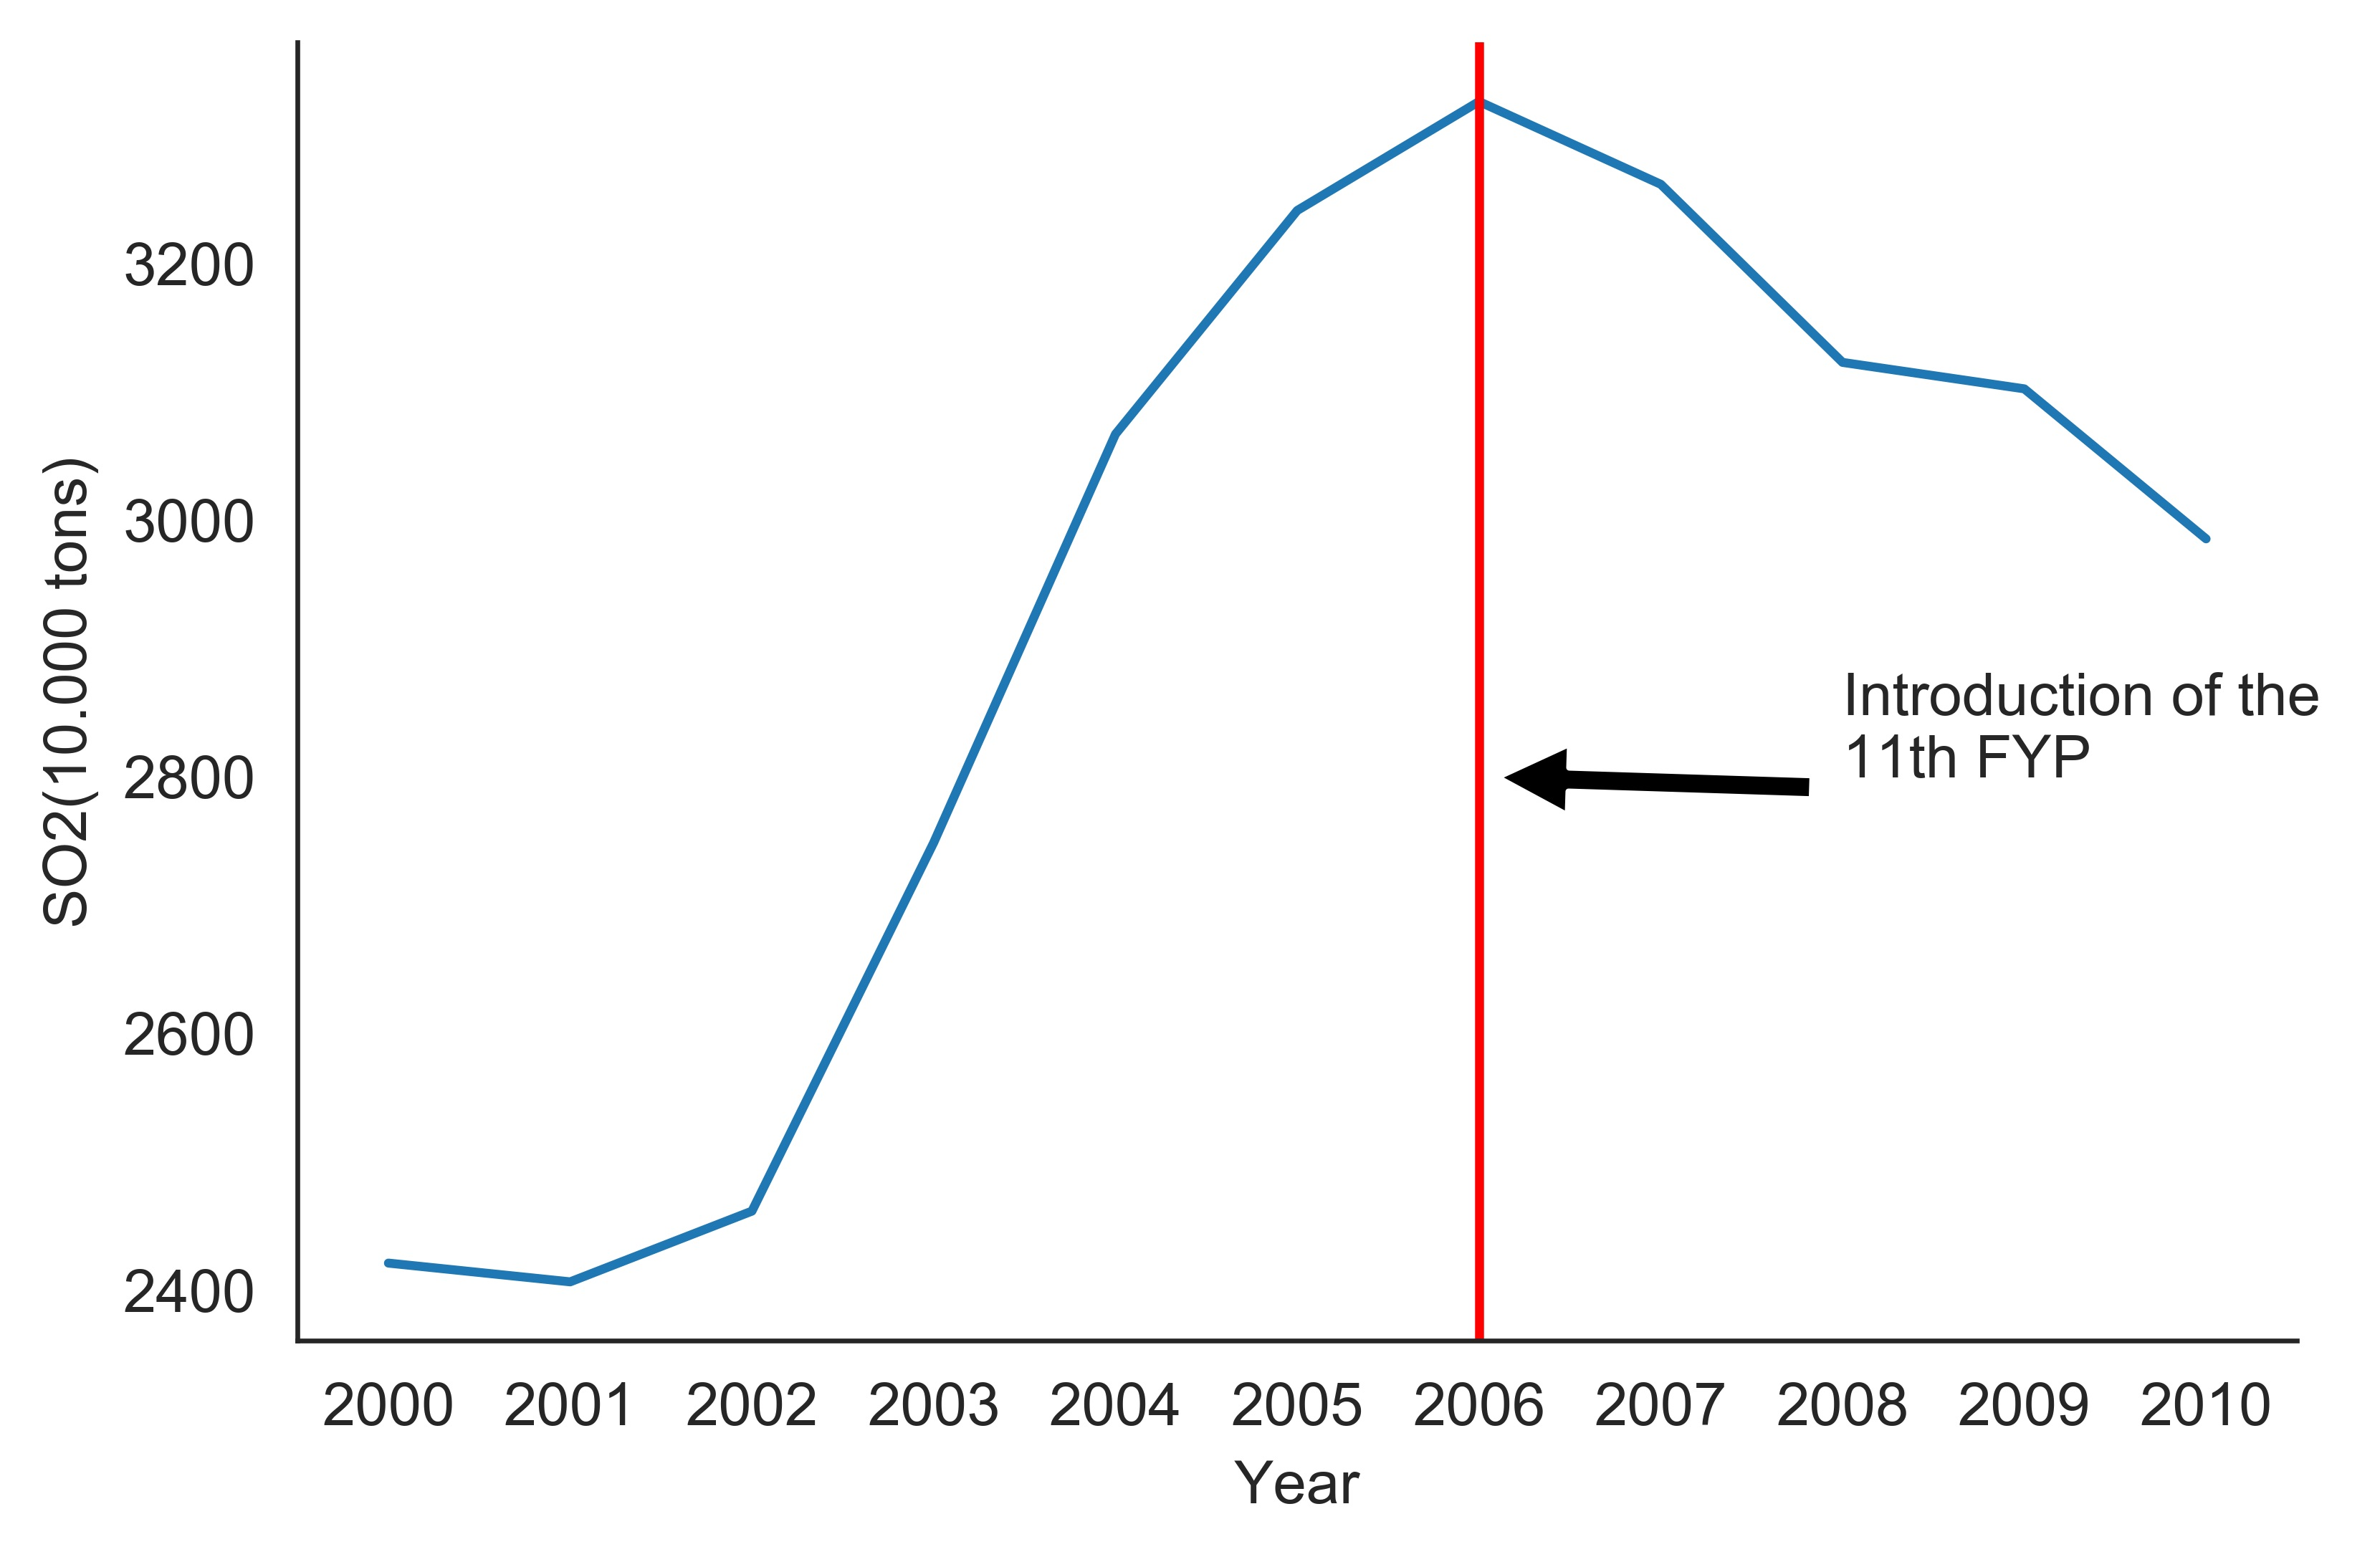
\includegraphics[width=0.5\textwidth]{fig_1}
    \caption{
    \small
    Emission of SO2 in China for the period 2000 to 2010.
    \textbf{Note}: The horizontal line represents the beginning on the 11th FYP. Starting from 2006, China introduced more environmental severity with an optimistic target of 10\% reduction of SO2 emission in 2010 compared with the level of 2005.\\
    \textbf{Source}: The SO2 emission data are from the \href{http://www.stats.gov.cn/english/Statisticaldata/AnnualData/}{China Statistical Yearbook (2000, 2010)}}
    \label{fig:figure1}
\end{figure}


\section{Policy \& environment} \label{sec:Policy}

The reform of China began in 1953 with the implementation of the FYPs by the central government, including economic development and social balance. The FYP is a set of national objectives that are initiated by the Communist Party of China and enforced by the local governments. Severe environmental incidents in the mid-1960s pushed the central government to address environmental issues more carefully. Although a decentralized system to control and prevent pollution has been operational since 1978, it has mainly been ineffective (\cite{Xu2009-yw}). Specific environmental regulations first appeared in the 9th FYP and they were strengthened afterward \footnote{The key features of environmental regulation are described in \cite{Xu2011-sw}.}. In the 10th FYP, a national objective of a 10\% reduction of the emissions of SO2 was established. To date, SO2 is one of the most significant sources of air pollution in China (\cite{Yan2017-le}). However, the bold objective of the 10th FYP failed, mainly for three reasons. First, banks have always provided credit to large industrial firms to promote industrialization, while paying little attention to the environmental degradation caused by the growth process (\cite{The_World_Bank2008-pn}). Second, the State Environmental Protection Administration (SEPA) was a weak regulatory agency (\cite{Stoerk2018-mx}). And third, local governments were not under threat of sanctions if they failed. The trade-off between growth and environmental warming is as binding in China as everywhere in the world. Up to the 11th FYP, economic growth, employment, and tax revenue were the key priorities of the local officials (\cite{Jiang2014-pf, Chen2018-ki}).

By the end of 2005, it was decided to enforce the 10\% mandate in the framework of the 11th FYP and more constraints were put in place at the local level. Economic growth and environmental objectives can be intertwined as long as the local government is responsible for the outcomes. A round of negotiations took place between the central government and the local government to allocate the pollution reduction mandates. Several different candidates were introduced in the computation of the target. The final pollution reduction estimate included economic growth, industrial structure, current pollution intensity, and geographic location (i.e., East, Central, West). In May 2006, the local government and the SEPA agency signed a contract to bind the reduction target ("The 11th Five-Year Plan: Targets, Paths and Policy Orientation")\footnote{The official statement is available \href{http://en.ndrc.gov.cn/newsrelease/200603/t20060323_63813.html}{here}.}. Following that statement, many provincial leaders decided to distribute the burden across cities (\cite{Liu2017-ib})\footnote{The government issued a document in 2006 with a clear guideline about the reduction allocation within-province. The formula is explicit: $\Delta C O D_{c, 05-10}=\Delta C O D_{p, 05-10} \times \frac{P_{c, 2005}}{\sum_{j=1}^{J} P_{j, 2005}}$.}. In July 2006, for instance, the provincial government of Shanxi disaggregated the SO2 reduction mandate down to the 11 cities.

One of the key elements of the regulation is that local leaders’ career opportunities are made dependent on the achievement of environmental objectives. A failure to meet the pollution reduction mandate leads to the dismissal of the official or a downgrade from his or her current position.

The Chinese government has shown its strong commitment to facilitate the tasks of the local authorities. In addition to the existing environmental laws and regulations, market-based policy instruments in favor of pollution reduction and environmental protection were introduced. Not only did the Chinese government pour enormous public investment into this problem but it also uses the financial markets to improve the environment. An improvement of the communication between SEPA and commercial banks allowed them to limit or even reject loans to firms infringing environmental laws (\cite{Oecd2008-pi}). Furthermore, credit administration institutions and SEPA developed strong ties that can restrain the access of high energy consumption input industries, and also promote environmentally friendly projects and emissions reduction. By the end of 2009, the total amount of investment geared toward the environment reached 1.33\% of China's GDP, which represents a yearly increase of 15\% since 2005. 

\section{Empirical Strategy} \label{sec:Empirical}

The main objective of our empirical strategy is to assess the effect of credit reallocation on the emission of pollution when banks face stringent environmental policies. We argue that banks allocate resources to firms that comply with environmental regulations and with the objectives of reducing pollution.

As mentioned in the section \ref{sec:Policy}, Policy and environment, in 2006 lawmakers assigned different levels of SO2  to cities, which should be met within the time span of the FYP. The spatial heterogeneity of this policy and the existence of a treatment year (before and after 2006) can be exploited to implement a difference-in-difference study and to identify the effect of stricter environmental policies. Our identification strategy also relies on financial dependency variability. We argue that firms who are dependent on banks are more likely to react to the new regulation when banks confronted with the new regulation can reallocate the credit away from polluting projects\footnote{This DDD strategy has been used in different papers to tackle the endogeneity problem. For more details about the related papers, please refer to \cite{Hering2014-af, Cai2016-br, Chen2018-ki, Shi2018-zk}.}.

This is reflected in the following equation, where we account for three levels of variability: 

\begin{equation} \label{eq:main}
SO2_{ckt} = \alpha\text{Financial Dependencies}_{k} \times Post_{t} \times \text{Reduction Mandate}_{c} + \beta X_{ckt} + \mu_{ct} + \gamma_{kt} + \delta_{ck} + \epsilon_{ckt}
\end{equation}

Where $SO2_{ckt}$ is the level of SO2 in city $c$, for industry $k$ and time $t$. The right-hand side of the equation contains three main variables, a set of control variables and fixed effects. $\text{Financial Dependencies}_{k}$ reflects the financial dependency of industry $k$ vis-a-vis banks. $Post_t$ is a dummy variable that takes the value of 1 when $t$ is above 2005, and otherwise is 0. This captures the two periods when the FYP takes place. $\text{Reduction Mandate}_{c}$ is the measure of stringent environmental policies in city $c$. We add three control variables usually found in the literature (\cite{Andersen2015-pa, Andersen2017-wf}), which are the $\text{total output}_{ckt}$, $\text{total fixed asset}_{ckt}$, and $\text{employment}_{ckt}$ aggregated at the city $c$, industry $k$ and time $t$. We use the log of the emission of SO2 and aggregate the different variables at the two-digit industrial level because this is the lowest level where $\text{Financial Dependencies}_{k}$ is available. The equation includes city-year fixed effect $\mu_{ct}$. It controls for all city characteristics that differ between cities through time, such as productivity, policies, wages. $\gamma{kt}$ is an industry-time pair fixed effect that captures the intrinsic features of each industry within time like the technological contents, subsidies. With $\delta{ck}$, we address the industry's invariant differences between cities. In our equation $\epsilon_{ckt}$ represents the error term.

Our strategy allows us to isolate the effect of stricter environmental policies before and after the 11th FYP with the inclusion of the fixed effects. Our identification compares the effect of stringent environmental regulation at different levels of financial dependencies on the emissions of SO2. The coefficient $\alpha$ is associated with the triple interaction term and it allows us to identify the effect of the treatment, namely the introduction of the 11th FYP, after 2006. We expect this term to be negative and significant. Cities with stricter targets should emit less SO2 during the second period of the analysis because the banks have more incentive to finance firms that respect environmental policies. In all regressions, the standard errors are two-way clustered by city and by industry. This enables spatial and serial correlation of the error term.

\section{Data and variables construction} \label{sec:Data}

\subsection{SO2 data sources} \label{sec:so2}

The Ministry of Environmental Protection (MEP) has collected the main data source of pollutants and wastes in China since 1980 \footnote{The name of the database is “Chinese Environmental Statistical Database (CESD”. The database is provided by the Ministery of Environmental Protection and kept very confidential.}. The MEP has monitored firms in 39 major industrial sectors that are considered as heavy polluters. These firms are asked to report basic information, such as company name, address, and output. They also answer a very detailed questionnaire about their emissions of major pollutants (e.g., wastewater, COD, SO2, industrial smoke, and dust). As reported in \cite{Wu2017-bl} and \cite{Jiang2014-pf}, this dataset contains about 85\% of the emissions of pollution from major pollutants in China. The MEP has implemented strict procedures, including unforeseen visits from experts, to ensure that these firms have not misreported their emissions. In our analysis, we have access to the SO2 statistics, a primary air pollutant, for 289 two digits industries, spread across 284 cities from 2002 to 2007.

The primary air pollutants reached a peak of emission in 2005 at 32.41 million tons of SO2 (figure \ref{fig:figure1}). Among the 522 cities monitored by the Chinese Ministry of Environment, about 400 had annual average SO2 levels that meet the Grade II national standard (0.06mg/m3) \footnote{China uses its own air quality standard, which is less stringent than the WHO’s standard. China's National Environmental Monitoring Center (CNEMC) has a real-time, hourly air quality data for major cities in China. The real-time data is available at \href{http://www.cnemc.cn/}{here}. Major air pollutants including SO2, NO2, and PM10 are monitored. To evaluate air quality, the Chinese government applies three classes. Class 1 means the yearly SO2 level is less than 0.02 mg/m3, or a daily average of less than 0.05mg/m3. Class 2 is less restrictive. The yearly average should not exceed 0.06 and a daily average of about 0.15. Class 3 is complacent with bad air quality. The yearly average can exceed 0.10 mg/m3, and the daily average is 0.25. By contrast, the \href{https://www.who.int/news-room/fact-sheets/detail/ambient-(outdoor)-air-quality-and-health}{WHO} recommends a daily average of less than 0.02mg/m3. For the records, exposure to high SO2 levels dangerously affects health. According to the WHO "SO2 can affect the respiratory system and the functions of the lungs and causes irritation of the eyes. Inflammation of the respiratory tract causes coughing, mucus secretion, aggravation of asthma, and chronic bronchitis and makes people more prone to infections of the respiratory tract.".} and 33 cities met the worst grade (0.10mg/m3). Two years after the 11th FYP was launched, the situation had slightly changed according to the Ministry of Environment in its annual report on the state of the environment in China \footnote{The report is available \href{http://english.mee.gov.cn/Resources/Reports/soe/soe2007/201}{here}.}. A total of 79\% percent of the audited cities met Grade II, which is two percentage points higher than in 2005. A towering achievement concerned the Grade III criteria, where less than 1.2\% of the cities were above the threshold and represents four percentage points less than 2005. The most polluted cities are located in Shanxi, Guizhou, Inner Mongolia, and Yunnan provinces. In table \ref{tab:appendixperiod} in the appendix, we computed the sum and average of the SO2 emission during both periods. Overall, we note that the average SO2 level is lower during the treatment period (10,714 - 10,432 tons).


\subsection{City reduction mandate} \label{sec:mandate}

The 11th FYP provides a general SO2 pollution reduction guideline for the provinces in China. The provincial leaders have a binding contract with the Ministry of Environment in which they bear the responsibility of any failure. To dilute the provincial objectives at a lower administrative level, the local government decided to include the cities. In a recent paper, (\cite{Chen2018-ki}) use an official document to estimate pollution reduction mandate at the city level. We replicate their methodology, which is based upon the following formula:

\begin{equation}
\Delta SO2_{c, 05 - 10}=\Delta SO2_{p, 05 - 10} \times \sum_{k=1}^{29} \mu_{k} \frac{\text { output value of industry } k \text { in city } c}{\text { output value of industry } k \text { in province } p}
\end{equation}

where, $c$ stands for city, $p$ for province and $k$ for the two digits industry. The left-hand side of the formula evaluates how much a city should reduce its SO2 emissions 2010 as compared with 2005. For example, Shanghai intended to reduce its SO2 emissions by 13,000 tons in 2010.

This estimate is computed by interacting with two components. The first component is the official province reduction mandate and is expressed in ten thousand tons \footnote{Province $p$ has the obligation to reduce the emission of pollution in 2010 by $x$ thousands of tons compared with the level in 2005.}. This measure is available for the 31 provinces of China. The second part is the share of industrial production $k$, in city $c$ over the total output of $k$ in province $p$. A weight, $\mu_k$, as the industry's proportion of total industrial SO2 emissions, is applied to account for the difference in SO2 intensity of each industrial sector.

We use the ASIF survey data to construct output share by industry for all the 298 cities of our dataset. The SO2 industry share $\mu_k$  is measured from the MEP dataset using the year 2005. Table \ref{tab:so2share} in the appendix reports the values of the 29 industrial share of $\mu$. For instance, the weight of \textit{Processing of Non-metallic Mineral Products} is 0.23, which is the largest in the sample, while in contrast \textit{textile} has a coefficient of  0.04. The average of the series is 0.034.

\begin{table}[hbt!]\centering
\resizebox{1\textwidth}{!}{
\begin{threeparttable}   
  \caption{\small SO2 emissions and control variables}

  \begin{tabular}{l*{6}{c}}
    
    \multicolumn{1}{l}{\textbf{Panel A: City-industry characteristics}} \\
    
    \toprule
     	 	 	 	 	
    & \multicolumn{6}{c}{} \\ 
    \hline
    & \multicolumn{1}{c}{All cities} & \multicolumn{1}{c}{Coastal}
    & \multicolumn{1}{c}{Southwest} & \multicolumn{1}{c}{Central}
    & \multicolumn{1}{c}{Northwest}& \multicolumn{1}{c}{Northeast}
    \\ 
    \hline 
    \midrule    
     
    SO2 & 10.619&	8.071	&18.349	&10.797	&14.493&	5.729\\
    (1.000 tons) & (38.967)&	(21.644)&	(62.603)&	(30.878)&	(69.606)&	(18.347)\\
    Output &9.31&	13.237	&7.882&	6.868&	6.412&	6.947\\
    (10 millions USD) & (15.264)&	(18.175)&(13.788)&(12.115)&(12.201)&(13.293)\\
    Fixed Asset & 70.319&	107.79&	44.952&	46.532&	44.799&	60.935\\
    (10 millions USD) &(129.37)&	(170.661)	&(84.336)	&(80.473)	&(75.504)&	(125.573) \\
    Employment &87.566&	151.077&	47.399&	55.559	&41.581&	51.515\\
    (10 millions) & (175.665)	&(261.522)&	(70.894)&	(75.958)&	(61.494)&	(80.275)\\

    \bottomrule     
    \\ %%% Create second table
    
    \multicolumn{1}{l}{\textbf{Panel B: City characteristics}} \\
    \toprule
    
    & \multicolumn{6}{c}{} \\ 
    \hline
    & \multicolumn{1}{c}{All cities} & \multicolumn{1}{c}{Coastal}
    & \multicolumn{1}{c}{Southwest} & \multicolumn{1}{c}{Central}
    & \multicolumn{1}{c}{Northwest}& \multicolumn{1}{c}{Northeast}
    \\ 
    \hline 
    \midrule 
    
    City Mandate &	1.245&	1.657&	1.658&	0.938&	0.728	&0.628\\
    (1.000 tons)&	(1.610)&	(1.731)&	(2.474)	&(1.078)	&(0.808)	&(0.739)\\
    \bottomrule
    
    Total Cities&	284&	87&	45&	80	&38	&34\\
    Observations &	25404&	9314&	3569&	6971&	2514&	3036\\
    \hline
  \end{tabular}
  \begin{tablenotes}
      \small
      \item Panel A provides a summary statistics for the variables that vary by city-industry-year. Panel B shows the key statistic for the variable varying with city only. The first row represents the average by variables. The standard deviations are presented in parentheses. \\
      Sources: MEP dataset and ASIF dataset. Author's own computation 
    \end{tablenotes}
\label{tab:table1}
\end{threeparttable}}
\end{table} 

Table \ref{tab:table1} gives a brief overview of the SO2 reduction target in the major area of China. Following \cite{Wu2017-bl}, we split cities between Coastal, Southwest, Central, Northwest, and Northwest \footnote{The province breakdown follows the paper of \cite{Wu2017-bl}. The Central provinces are Anhui
Henan, Hubei, Hunan, Jiangxi, and Shanxi. The Coastal provinces are Beijing, Fujian, Guangdong, Hainan Hebei, Jiangsu, Shandong, Shanghai, Tianjin, and Zhejiang. The Northeastern provinces are Heilongjiang, Jilin, Liaoning. Northwest are Gansu, Inner Mongolia, Ningxia, Qinghai, Shaanxi, and Xinjiang. The Southwestern parts are Chongqing, Guangxi, Guizhou, Sichuan, Yunnan, and Xizang.}. The Coastal area of China is composed of 10 provinces and has a total of 87 cities. This area is the wealthiest part of China, and is where most of the national production and foreign investment take place. The Southwestern area has five provinces and 45 cities, while the Central area has six provinces and 80 cities. The Northern part of China is split into the Western area with six provinces and 38 cities and the Eastern area with three provinces and 34 cities. The Coastal and Southwestern parts of China have to reduce pollution by 16,600 tons, on average, before the end of the 11th FYP. The Central part of China is confronted with an objective of 9,400 tons, closely followed by the Northwest and Northeast.

\subsection{A measure of sector-level reliance on external finance} \label{sec:fin}

To meet the production level, firms need to finance a fraction of the costs (fixed and variable). We use the industry’s external finance dependency, which is defined as the exposure of industry to the banks. The computation of the industry’s external finance dependency is straightforward—it is the share of capital expenditure not financed with cash flow from operations. Previous works have used US data to proxy for the exposure to external finance (\cite{Rajan1998-tn, Claessens2002-mj, Kroszner2007-gt}) and in the context of China (\cite{Jarreau2014-lb, Manova2015-zk, Fan2015-bm}). We use the Chinese data and replicate the methodology proposed by \cite{Fan2015-bm}, who use the ASIF dataset during the years 2004–2006 to aggregate the capital expenditure and cash flow at the two digits industrial level. \cite{Fan2015-bm} argue \footnote{Unlike the US methodology, which uses the median over time, the authors use the aggregate value from the Chinese data because about 68\% of the observations have 0 capital expenditure.} that the financial pattern between the US and China is almost similar. Tobacco is the least vulnerable sector in the US, while it ranks second in China. The leather products industry is the second least vulnerable in the US and the fifth least vulnerable in China. Table \ref{tab:so2share} in the appendix gives the value of financial dependence for the 29 industries in China. The average value is -.57, and industries with a high technological requirement are also the most vulnerable. The \textit{Petroleum} industry and \textit{Processing of Nuclear Fuel} industries are at the bottom of the table, stressing their high reliance on credit.

\subsection{City industry variables: control} \label{sec:control}

Recent papers have demonstrated the role of the factors of production on the deterioration of the environment (\cite{Cole2003-ad, Cole2008-pj}). Furthermore, capital intensity positively affects the emission and intensity of pollution (\cite{Hering2014-af, Andersen2017-wf}). In addition, large industries generate more emissions of SO2. The National Bureau of Statistics of China (NBS) collects manufacturing data for all non-state-owned-enterprise with sales above RMB 5 million and state-owned-enterprise (SOE). The survey contains detailed information about the name, address, four-digit CIC industry classification, ownership, and financial variables, including output, sales, fixed assets. This dataset is reliable for at least two reasons. First, since 1995 the NBS has used the firms’ survey data to compute metrics such as GDP. Second, firms do not have incentives to misreport the numbers. According to \cite{Chen2018-ki}, the NBS is not allowed to share information with other agencies (e.g., tax agency, government, etc.). The NBS uses its industrial classification to sort firms by sectors. Given that our data started in 2002 and ended in 2007, we can use the 2002 GBT classification for each year of our sample data. The financial dependency variable is computed at the two-digit industrial level. To stay consistent with the financial dependency variable, all of the industrial variables are computed at the two digits classification.  We aggregate the total output by year and city for all the two-digit industries. We also compute the total employment at the city-industry-year level. Finally, the ASIF dataset gives the yearly total net fixed asset by firms. We use this information to compute the city-industry-year total fixed asset. Table \ref{tab:table1}, panel A, shows the basic metrics about total output, fixed asset, and employment for all the cities and also the spatial location.

\subsection{A first glance at the structure of Chinese SO2 emitting industries}

The level of SO2 emissions between sectors in China has remarkable variations. The objective of this paper is to disentangle the different levels of pollution when a sector faces different borrowing constraints. A bank’s incentive to finance a project is motivated not only by the commercial aspect but also from the environmental pressure imposed with the local government. More precisely, cities are imposed by different levels of environmental severity, which is translated into maximum SO2 emissions allowed by the end of the 11th FYP, as shown in Figure \ref{fig:figure2}.

\begin{figure}[ht]
    \centering
    \textbf{Actual against targeted pollution reduction}\par\medskip
    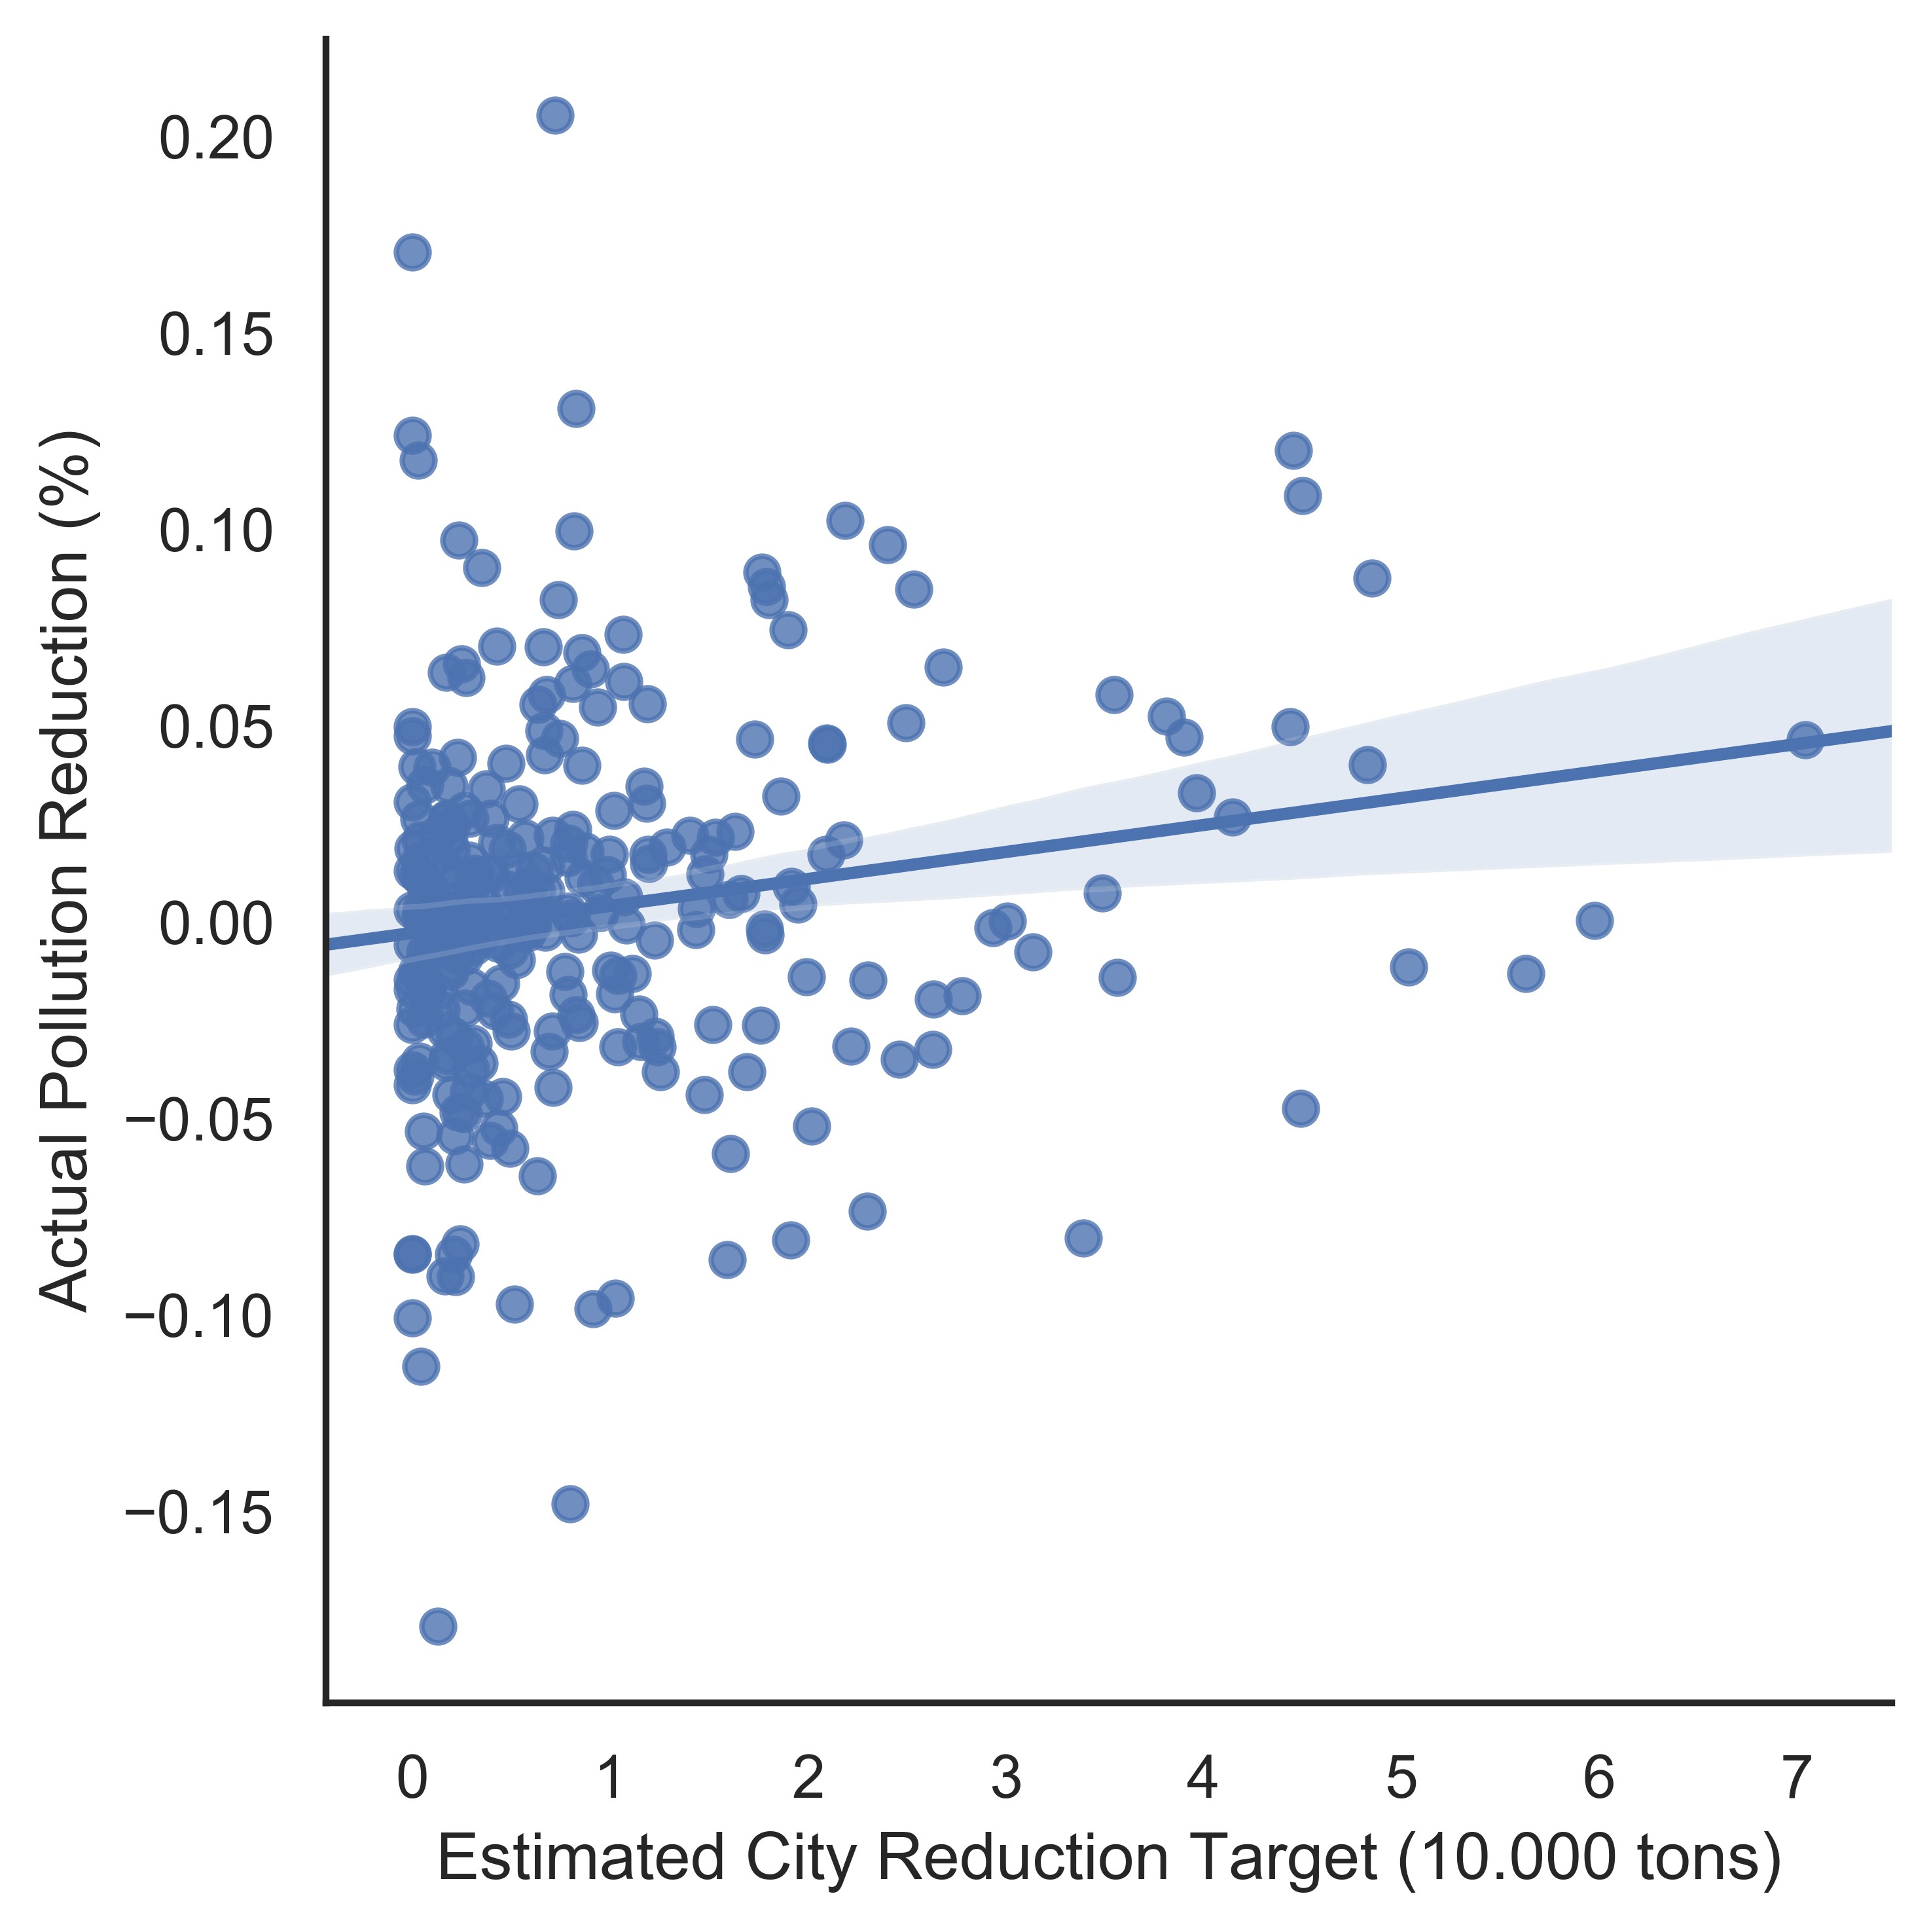
\includegraphics[width=0.5\textwidth]{fig_2}
    \caption{
    \small
    SO2 Reduction Targets and Actual Pollution Reduction, at the city level, are estimated according to the methodology proposed in section \ref{sec:mandate}.
    \textbf{Note}: Points in the figures represent cities. Y-axis is Log(SO2 emission in 2005 - SO2 emission in 2007)/(SO2 emission in 2005)). The line represents the fitted values. A positive trend indicates that cities with stringent reduction mandate managed to reduce the level of SO2 emitted in 2007 compared with 2005. \\
    \textbf{Source: MEP Dataset}. Author's own computation}
    \label{fig:figure2}
\end{figure}

We plot the relationship between the city’s reduction target and the variation of SO2 emissions for 2005 and 2007 \footnote{Variation is computed as follows: $Log(\text{SO2 emission in 2005 - SO2 emission in 2007})/(\text{SO2 emission in 2005}))$.}. The x-axis represents the reduction target formulated by the local government and implemented by the cities. Section \ref{sec:mandate}, provides more details about the formula that we used to estimate the city reduction mandate. For the y-axis, we computed the log difference of SO2 emissions in 2005 and 2007. Values above 0 indicate a reduction of SO2 emissions in 2007 compared with 2005. For the following graphs, we use the same y-axis variable. The positive line shows that cities with stringent environmental regulations put more effort into fighting pollution. Most of the cities decreased their emissions in 2007 when compared to 2005, with a faster reduction for cities under environmental pressure. In figure \ref{fig:figure3}, we plot the industry financial dependencies against the industry changes in pollution emission between 2005 and 2007. $\text{Financial dependency}$ is borrowed from the paper of \cite{Fan2015-bm}, who computed the borrowing constraints for 29 sectors in China. Sectors with large values need to find funding from financial players. If $\text{Financial Dependency}$ is high, then the industry is more financially vulnerable and has a larger reliance on external funding. Industries exposed to bank funding managed to lower their emissions of SO2 at a faster speed. This suggests that the banks have reoriented loans in favor of sustainable finance. 

\begin{figure}[ht]
    \centering
    \textbf{Reliance of financial dependency and success of reduction pollution}\par\medskip
    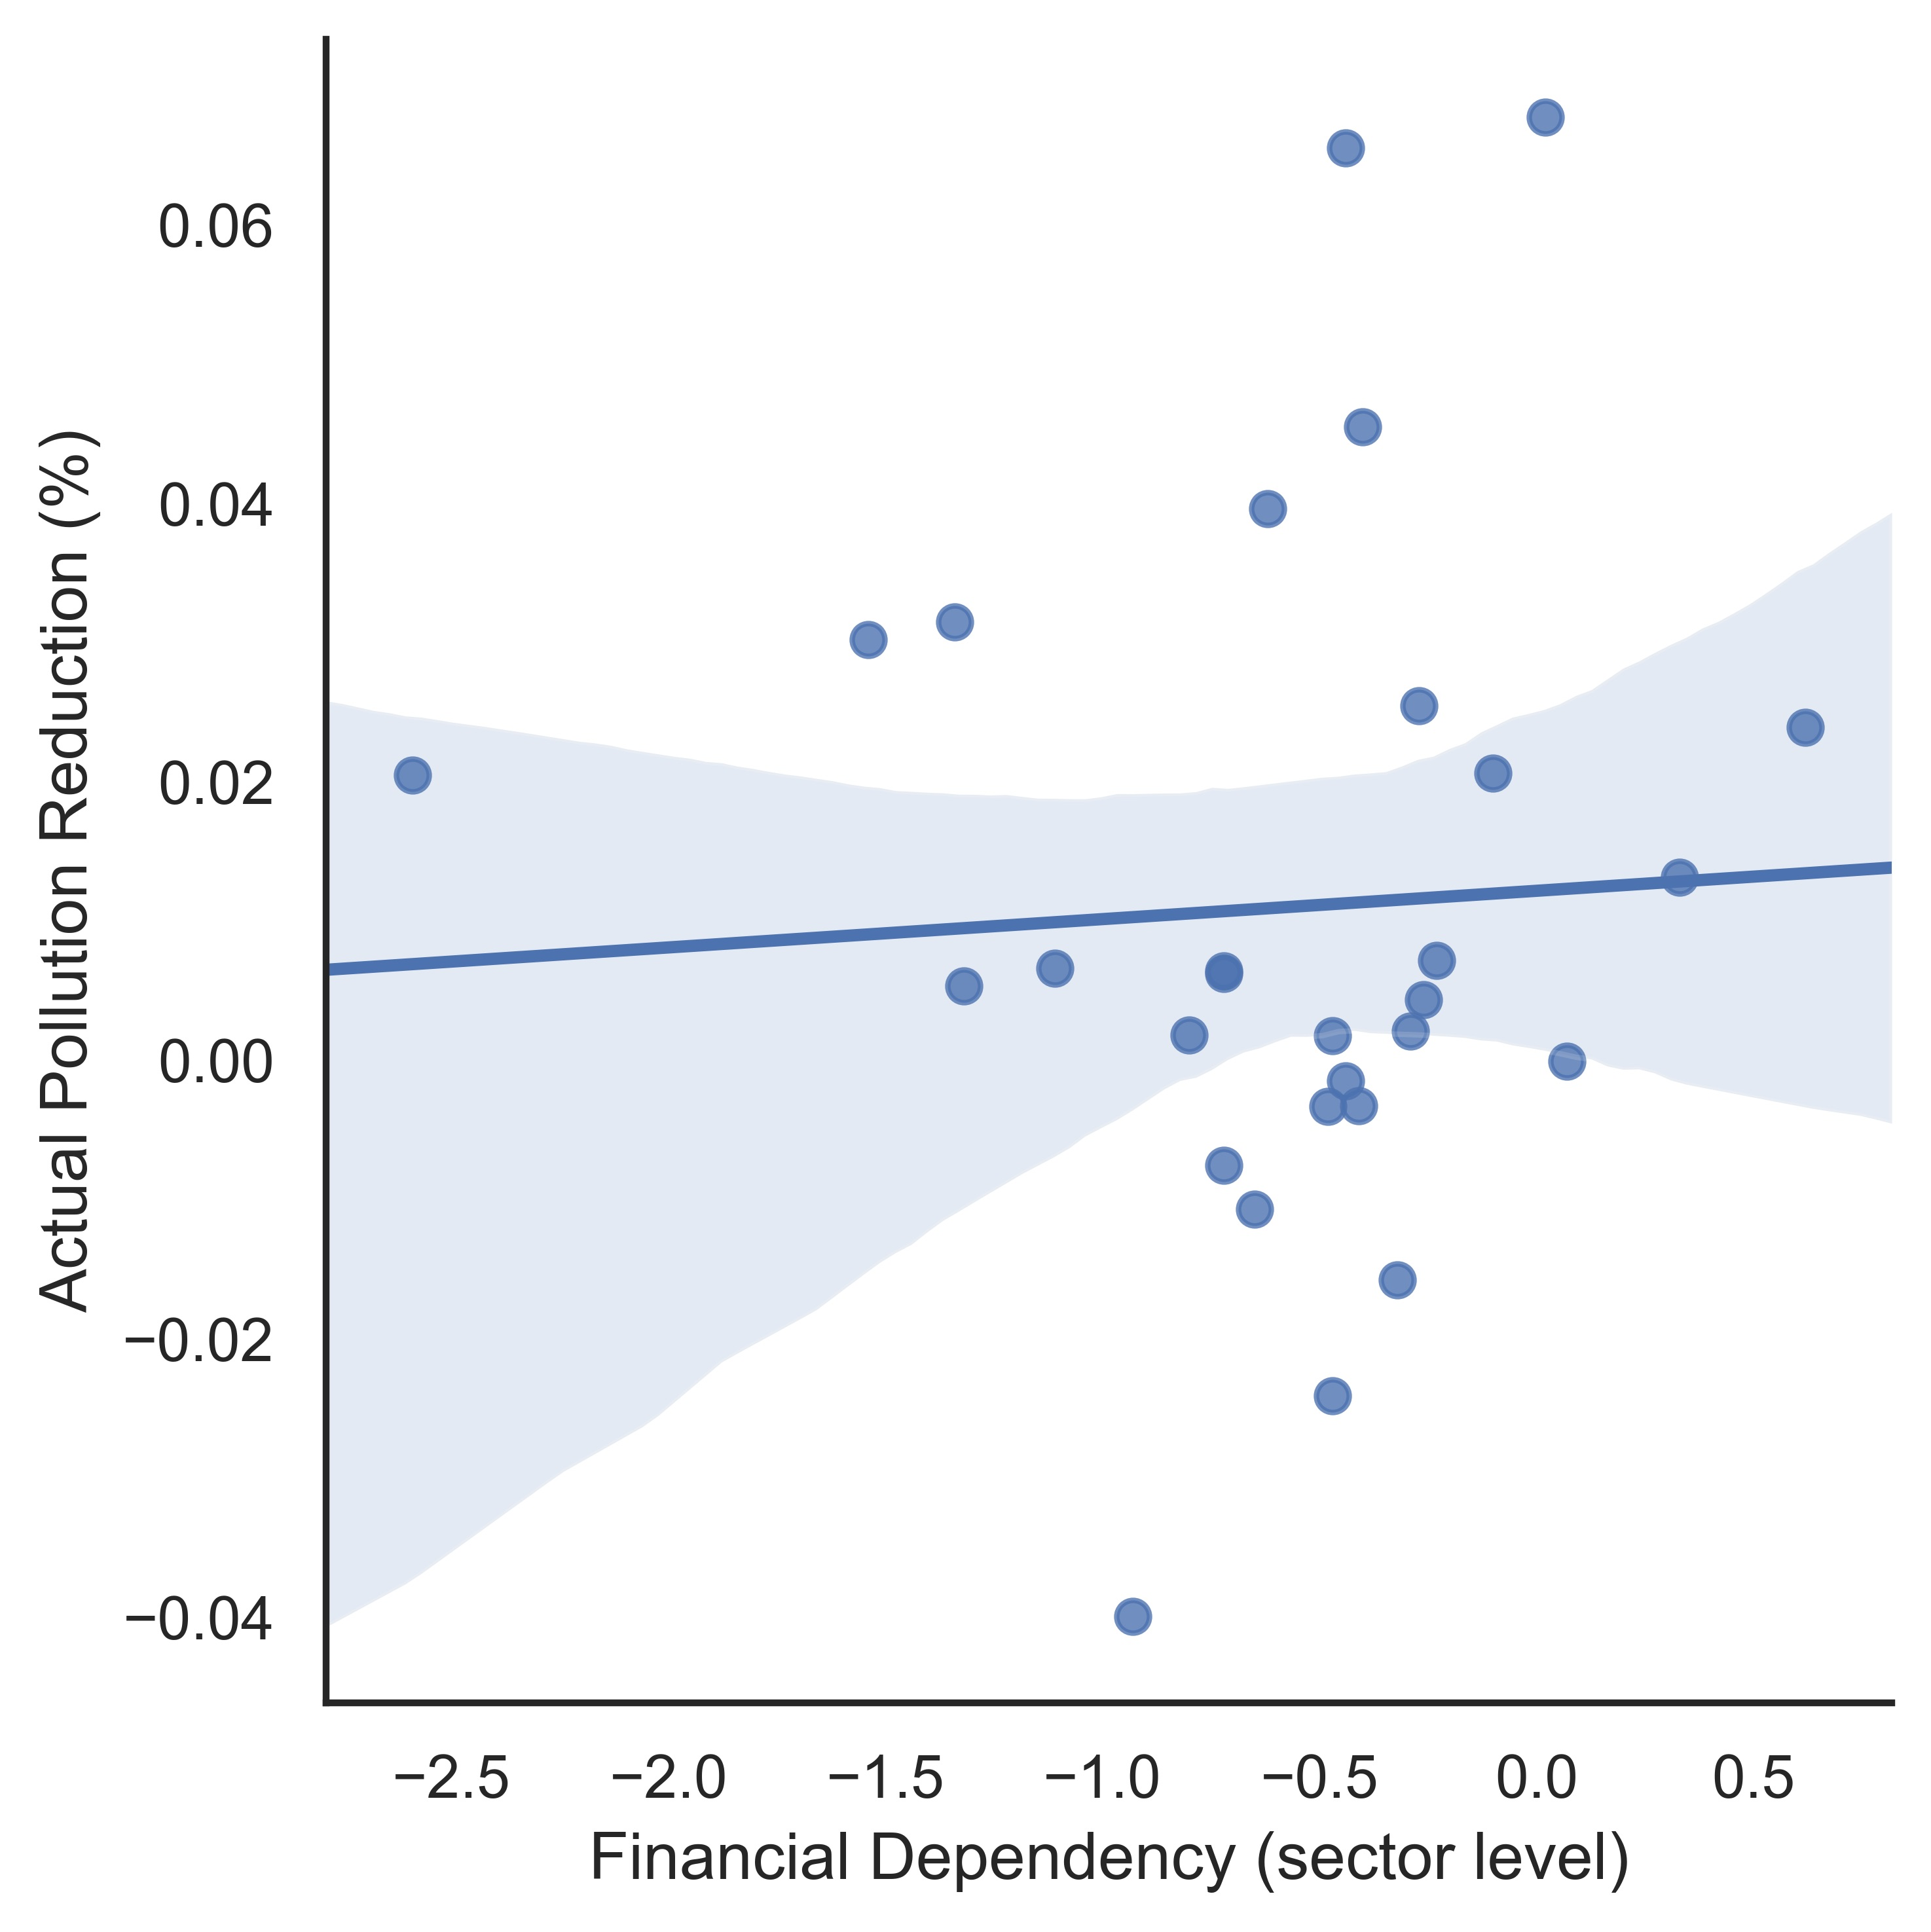
\includegraphics[width=0.5\textwidth]{fig_3.jpg}
    \caption{
    \small
    Financial Dependencies by sector and Actual Pollution Reduction.
    \textbf{Note}: Points in the figures represent 29 CIC sectors. Y-axis is Log(SO2 emission in 2005 - SO2 emission in 2007)/(SO2 emission in 2005)). The line represents the fitted values. A positive trend indicates that sectors relying on banks’ funding were more successful in reducing the level of SO2 emitted in 2007 compared with 2005. \\
    \textbf{Sources}: MEP Dataset and \cite{Fan2015-bm}. Author's own computation}
    \label{fig:figure3}
\end{figure}

Our empirical approach links the financial dependencies with the stringency of the local environmental regulation to understand the industrial and local changes in the emissions of pollution. Figure \ref{fig:figure4} analyses the variations of SO2 emission by financially constrained sectors of two cities with different environmental mandates. The city of Tangshan belongs in the top decile of environmental severity. The city of Xiamen is in the third decile. Both cities share similar GDP characteristics \footnote{Tangshan is a largely industrial prefecture-level city in the northeast of Hebei province. Tangshan’s GDP was about 10,744,000 RMB in 2005. Xiamen is a port city on China’s southeast coast, across the strait from Taiwan. It encompasses two main islands and a region on the mainland. The GDP of Xiamen was around 10,065,830 RMB in 2005.}.

\begin{figure}[ht]
    \centering
    \textbf{Financial dependencies and two economically identical cities with different environmental regulations}\par\medskip
    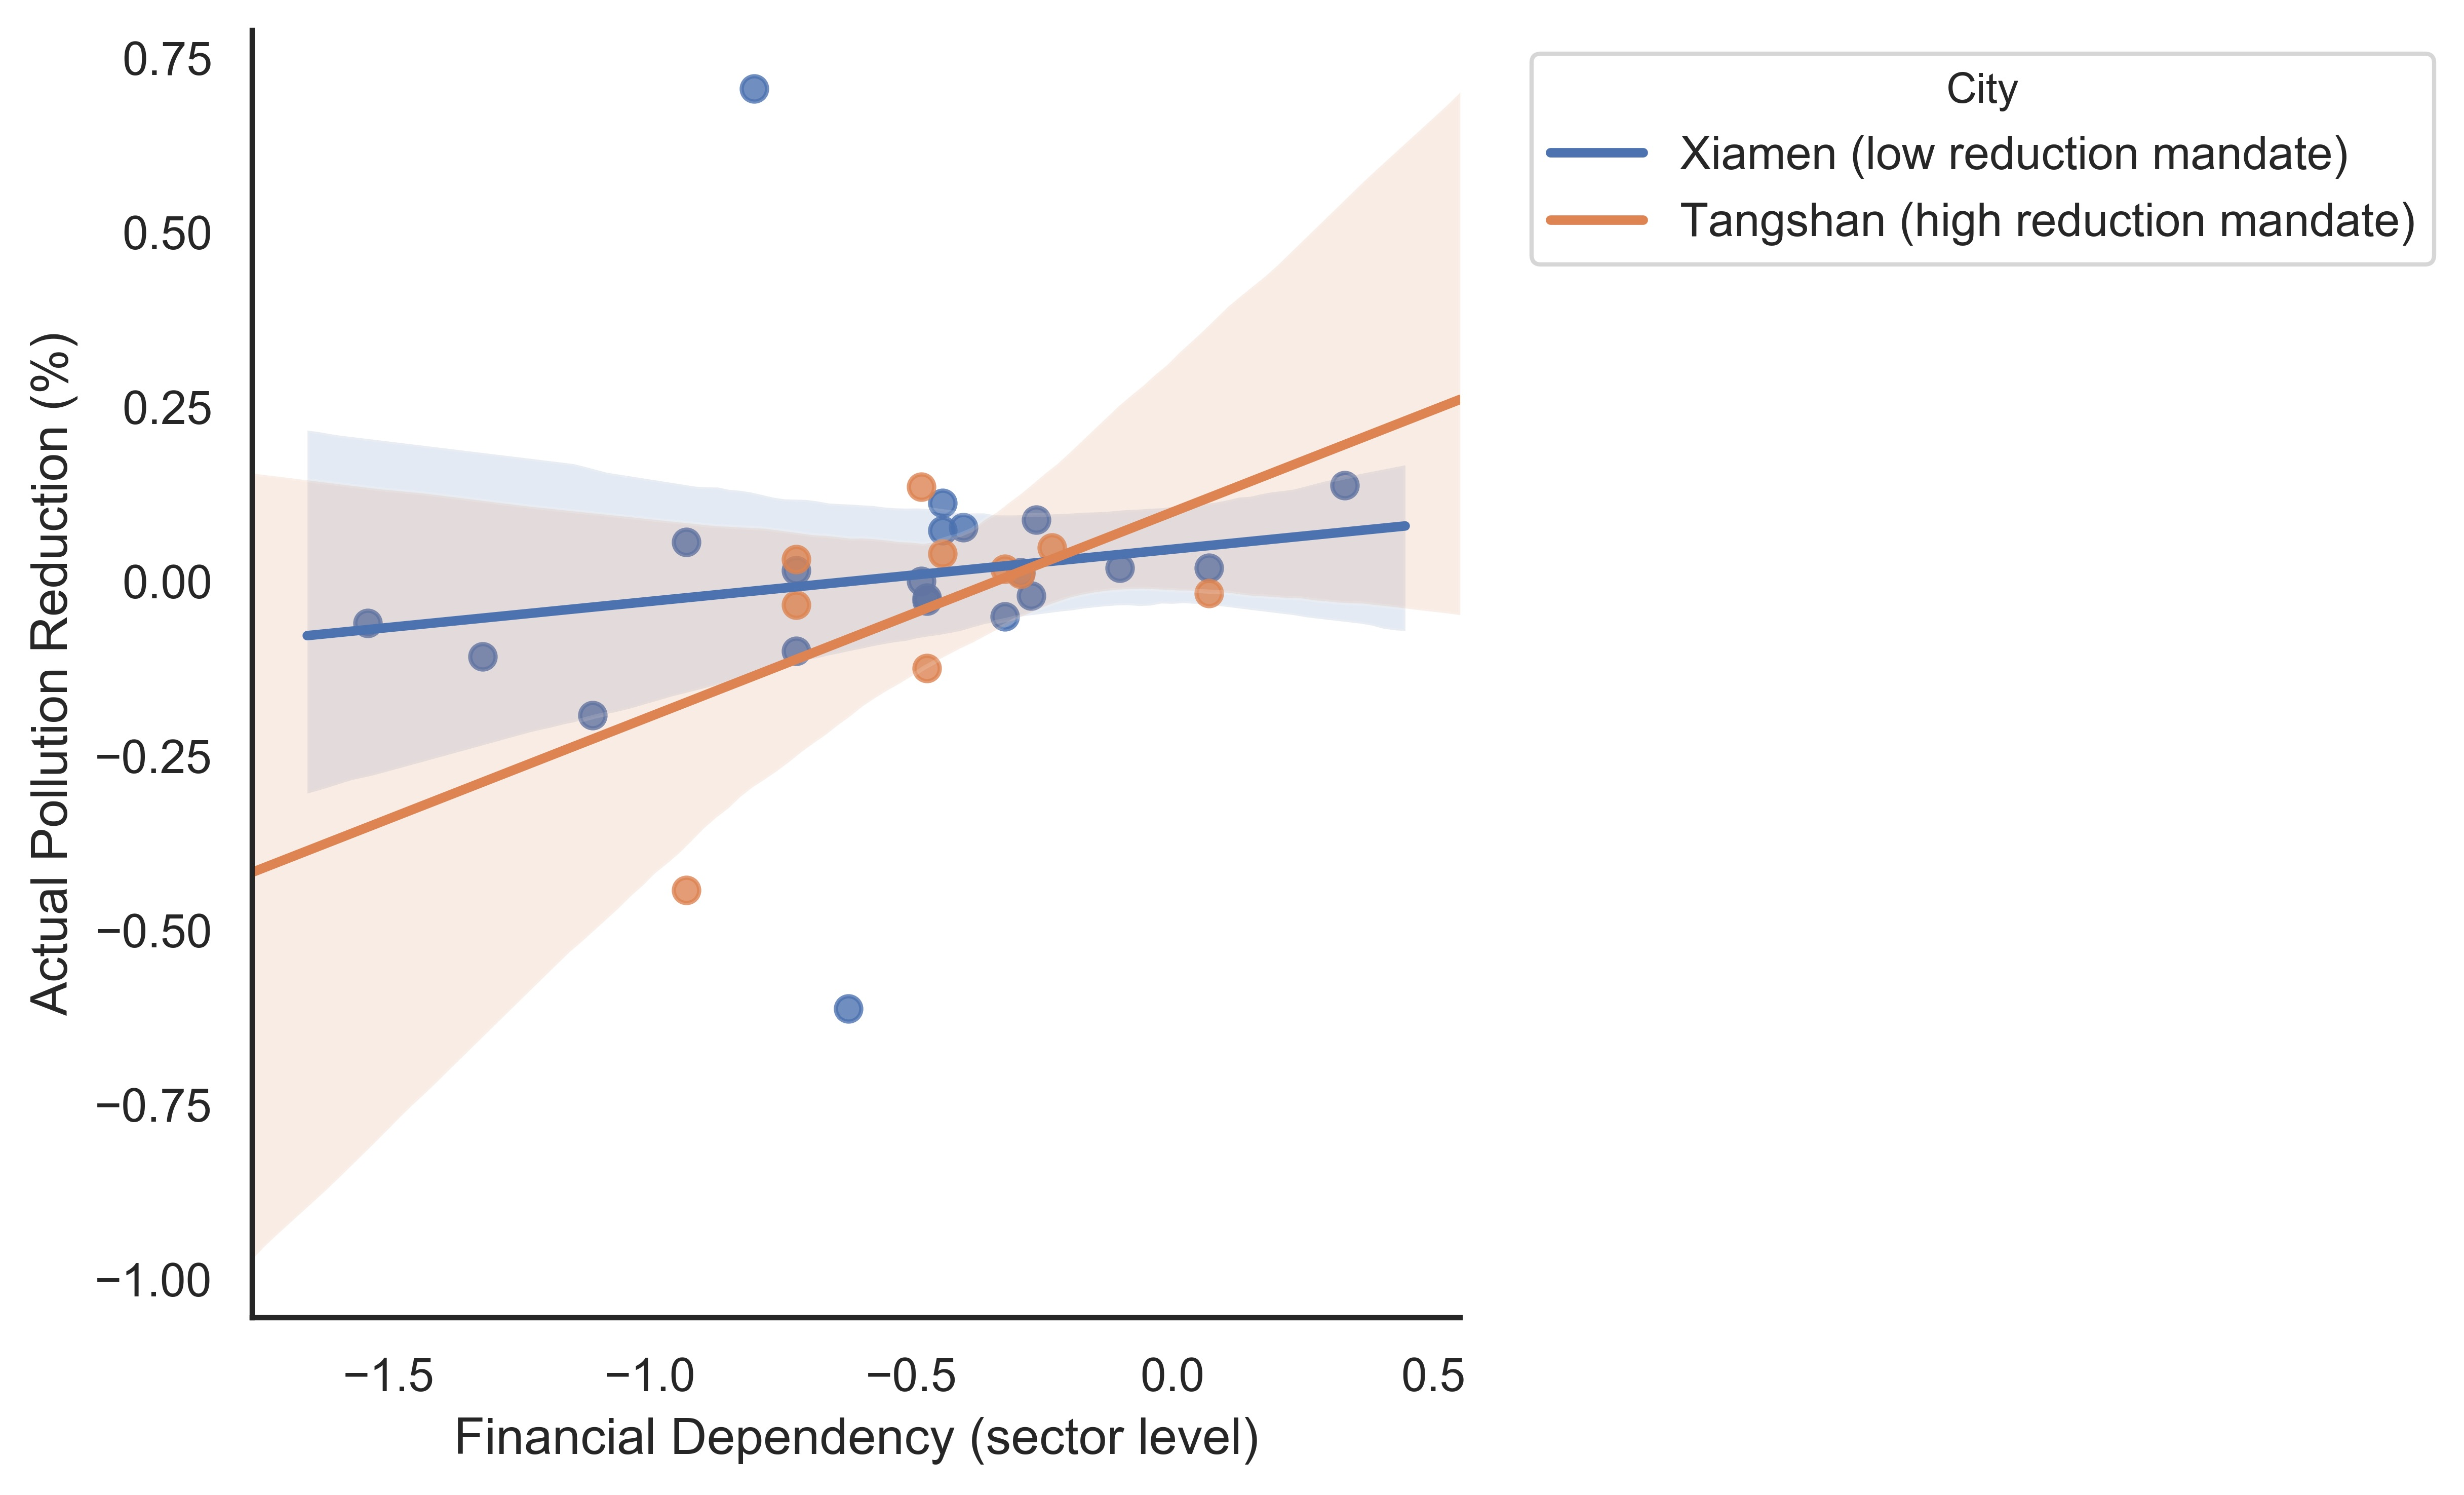
\includegraphics[width=0.7\textwidth]{fig_4.jpg}
    \caption{
    \small
    Financial Dependencies by sector and Actual Pollution Reduction for two similar cities facing different reduction mandates.
    \textbf{Note}: Points in the figures represent 29 CIC sectors. Y-axis is Log(SO2 emission in 2005 - SO2 emission in 2007)/(SO2 emission in 2005)). The line represents the fitted values. A positive trend indicates that sectors relying on banks’ funding managed to reduce the level of SO2 emitted in 2007 compared with 2005. Both cities are similar in terms of GDP, Tangshan has to comply with an higher mandate. As a result, the slope of the line is steeper, suggesting that the impact of the financial vulnerability is stronger.\\
    \textbf{Sources}: MEP Dateset and \cite{Fan2015-bm}. Author's own computation
    }
    \label{fig:figure4}
\end{figure}

In line with our expectations, the contribution to lower SO2 emission is stronger for financially dependent sectors in cities with stringent mandates. This implies that the banks have more incentives to screen sustainable projects when there is local environmental pressure.

\section{Results of the effect of financial dependencies on the emission of SO2} \label{sec:result}

\subsection{Main results}

Our primary interest is to assess the impact of credit access on the emissions of SO2 in the context of tighter environmental regulations. Table \ref{tab:table2} reports the baseline regression (equation \ref{eq:main}). Columns 1 and 2 focus on the log of SO2 emissions at the city-industry-year level. Columns 3 and 4 focus on the log of SO2 emission divided by the value-added at the city-industry-year level, which is called \textit{SO2 intensity}. All of the regressions include an extensive range of fixed effects to control for time, city, and industry characteristics. 

\begin{table}[hbt!]\centering
\resizebox{1\textwidth}{!}{
\begin{threeparttable}   
  \caption{\small The effect of environmental regulation and financial dependency on the emission of SO2, baseline regression}

  \begin{tabular}{l*{4}{c}}
  
    \toprule
     
    & \multicolumn{4}{c}{} \\ 
    \hline
    & \multicolumn{2}{c}{Ln SO2} & \multicolumn{2}{c}{Ln SO2 intensity} \\
\\[-1.8ex] & (1) & (2) & (3) & (4)\\ 
\hline 

  $\text{Financial dep.}_k$ x Post x $\text{SO2 mandate}_c$ & $-$0.354$^{*}$ & $-$0.514$^{**}$ & $-$0.415$^{*}$ & $-$0.601$^{***}$ \\ 
  & (0.208) & (0.200) & (0.213) & (0.207) \\
  $\text{Ln output}_{ckt}$ & 0.509$^{***}$ & 0.486$^{***}$ & 0.473$^{***}$ & 0.456$^{***}$ \\ 
  & (0.027) & (0.029) & (0.026) & (0.031) \\ 
  $\text{Ln fixed asset}_{ckt}$ & 0.034 & 0.049$^{*}$ & $-$0.221$^{***}$ & $-$0.214$^{***}$ \\ 
  & (0.030) & (0.026) & (0.040) & (0.035) \\ 
  $\text{Ln employment}_{ckt}$ & 0.082$^{**}$ & 0.076$^{**}$ & $-$0.548$^{***}$ & $-$0.547$^{***}$ \\ 
  & (0.035) & (0.038) & (0.047) & (0.055) \\  
\midrule

City-year fixed effects & Yes & Yes & Yes & Yes \\ 
Industry-year fixed effects & Yes & Yes & Yes & Yes \\ 
City-industry fixed effects & Yes & Yes & Yes & Yes \\ 
Observations & 25,404 & 18,509 & 25,404 & 18,509 \\ 
R$^{2}$ & 0.889 & 0.866 & 0.869 & 0.860 \\  

\bottomrule
  \end{tabular}
  \begin{tablenotes}
      \small
      \item SO2 intensity is computed as the total SO2 emission by city-industry-year divided by value added. SO2 city mandate measures the total amount of SO2 a city needs to reduce by the end of the 11th FYP. Columns 2 and 4 exclude the top and bottom 4 most polluted sectors in 2002.
 * Significance at the 10\%, ** Significance at the 5\%, *** Significance at the 1\%. Heteroskedasticity-robust standard errors in parentheses are two-way clustered by city and by industry.
    \end{tablenotes}
    \label{tab:table2}
\end{threeparttable}
}
\end{table}

The first row of table \ref{tab:table2} represents our coefficient of interest, the interaction between the sector reliance on external financing, environmental regulation, and the period of the 11th FYP. All of the coefficients are negative and significant. The coefficient of the triple interaction term is larger for \textit{SO2 intensity}, which suggests that the environmental performance has to be scaled down according to the production scale. In columns 2 and 4, we ensure that extreme sectors do not drive our results. Therefore, we removed the top and bottom polluted sectors in 2002 \footnote{We excluded the following four least (most) polluted sectors: Furniture, Artwork and Other Manufacturing, Printing, Reproduction of Recording Media, Electrical Machinery and Equipment, Smelting and Pressing of Non-ferrous Metals, Raw Chemical Materials and Chemical Products, Smelting and Pressing of Ferrous Metals and  Non-metallic Mineral Products.}. The coefficients of SO2 and SO2 intensity become larger and they remain significant at 5\% and 10\%, respectively. Overall, these results suggest that in a highly regulated area, banks tend to re-allocate credits to firms that obey the environmental policies.

The coefficient in column 1 means that the requirement of a  reduction by one standard deviation above the mean (which represents 1500 tons of SO2) leads to a reduction of pollution emission by 3.54\%. The mean pollution being set equal to 11,000 tons in 2005, this implies a reduction of S02 emissions by 4000 tons (11.000 times 0.0354). Researchers have estimated that the external damage cost of one ton of sulfur dioxide to be equivalent to \$7228 \footnote{This number, which represents the cost of SO2 emitted per ton in different years, varies across studies. Greenpeace estimates the cost of SO2 per ton to be \$4356 for non-European countries. According to the OECD and for a sample of  14 European countries, it is about \$9557. For the European Union, which refers to a city of 100,000 population, it reaches \$7770. Therefore, we take the average of these three values in 2007 for the year  2007 and we use the euro/USD exchange rate of 1.11.}. An increase of the reduction mandate by 1 standard deviation can therefore be valued at 29 million USD per year (7228 x 4000).  

To illustrate the difference between a sector that is financially dependent on credit relative to a sector that is not, we compare the value of the 10th percentile of the variable $\text{Financial Dependencies}$ and the 90th percentile. The 10th percentile in the data corresponds to the \textit{Leather and fur} industry, and the 90th is \textit{Paper}. We set the increase of SO2 reduction mandate to 1.500 tons (roughly one standard deviation), and $\alpha= -.354$. Taking everything being equal, the key point is that the differential impact between the 90th and 10th percentiles of financial dependence \footnote{The value of the 10th quantile for  $\text{Financial Dependencies}$ is $-1.11$ and for the 90th quantile is 0.07.} is equal to -7.19\% for an increase of 1.500 tons of SO2 mandate, which is strongly negative and significant \footnote{The quantile point estimate formula is the following: $value \times \alpha \times (\text{Financial Dependencies}_{90^{th}} - \text{Financial Dependencies}_{10^{th}})$. The point estimate is calculated by $1500/10000 * -.354 * (0.03 + 1.324 )) * 100$ . $-.354$ is the $\alpha$ coefficient from table \ref{tab:table2}, column 1.}.

In addition to the triple interaction terms and the fixed effects, our specification controls for variables that vary across time, city, and industry. We include the output, fixed asset, and employment variables aggregated at the city, industry year level. Rapid economic development has severely degraded the environment. The coefficient of the output is highly significant and positively correlated with SO2 and SO2 intensity, which puts high pressure on the environment. Employment and fixed assets are positively correlated with SO2 and negatively correlated with SO2 intensity. Including these variables does not affect our coefficient of interest.

\subsection{Testing for parallel trends}

Our identification strategy is biased if some omitted circumstances are driving the allocation of credit toward more responsible firms before the 2006 policy. For instance, as early as in 2005, cities were given policy recommendation for the production based on the level of SO2. Therefore, they could have anticipated the mandatory requirements of the 11th FYP by implementing them before 2006. To ensure that our specification does not pick up such a pre-trend anticipation effect, we replicate the estimates from table \ref{tab:table2} while changing the $Post$ variable with year-dummies set equal to one over the time span 2002–2007.

\begin{table}[hbt!]\centering
\resizebox{1\textwidth}{!}{
\begin{threeparttable}   
  \caption{\small The effect of environmental regulation and financial dependency on the emission of SO2, testing the parallel trend assumption}

 \begin{tabular}{l*{2}{c}}
    
    %\multicolumn{1}{l}{\textbf{\small The effect of environmental %regulation and financial dependency on the emission of SO2, %testing the parallel trend assumption}} \\
    
    \toprule
     
    & \multicolumn{2}{c}{} \\ 
\hline
& \multicolumn{1}{c}{Ln SO2} & \multicolumn{1}{c}{Ln SO2 intensity} \\ 
\\[-1.8ex] & (1) & (2) \\ 
\hline
   $\text{Financial dep.}_k$ x Year 2003 x $\text{SO2 mandate}_c$ & $-$0.236 & $-$0.240 \\ 
  & (0.225) & (0.235) \\ 
  $\text{Financial dep.}_k$ x Year 2004 x $\text{SO2 mandate}_c$ & $-$0.276 & $-$0.288 \\ 
  & (0.257) & (0.256) \\ 
  $\text{Financial dep.}_k$ x Year 2005 x $\text{SO2 mandate}_c$ & $-$0.383 & $-$0.445 \\ 
  & (0.242) & (0.282) \\ 
  $\text{Financial dep.}_k$ x Year 2006 x $\text{SO2 mandate}_c$ & $-$0.567$^{*}$ & $-$0.641$^{*}$ \\ 
  & (0.344) & (0.333) \\ 
  $\text{Financial dep.}_k$ x Year 2007 x $\text{SO2 mandate}_c$ & $-$0.594$^{**}$ & $-$0.682$^{**}$ \\ 
  & (0.290) & (0.329) \\  
\midrule
City-year fixed effects & Yes & Yes  \\ 
Industry-year fixed effects & Yes & Yes  \\ 
City-industry fixed effects & Yes & Yes  \\ 
Observations & 25,404 & 25,404 \\ 
R$^{2}$ & 0.889 & 0.869 \\  
\bottomrule
  \end{tabular}
  \begin{tablenotes}
      \small
      \item The year 2002 is the omitted category. SO2 intensity is computed as the total SO2 emission by city-industry-year divided by value added. All columns controls for the output, fixed asset and employment computed at the city, industry, year. \\
      * Significance at the 10\%, ** Significance at the 5\%, *** Significance at the 1\%. Heteroskedasticity-robust standard errors in parentheses are two-way clustered by city and by industry.
    \end{tablenotes}
    \label{tab:table3}
\end{threeparttable}}
\end{table}

Table \ref{tab:table3} displays the results for each year. All of the coefficients before the launch of the 11th FYP are negative but not significant, which validates our strategy of identification. The coefficients become significant in 2006 and increase in size afterward, which implies that the policy is reinforced over time. Similar results hold with the variable SO2 intensity, as reported in column 2. All of the estimates are obtained from specifications that control for output, fixed asset, and employment computed at the city, industry, and year.


\subsection{Heterogeneous effect}

We have provided evidence of the average effect of financial reliance on external credit on the emission of SO2. In this section, we investigate whether this average effect differs according to firms’ ownership and size. It is well-known that China's political pecking order of firms is enforced through the systematic misallocation of financial resources (\cite{Dollar2007-dr}), and that credit allocation is biased in favor of state-owned enterprises (\cite{Huang2003-oa, Brandt2003-hu, Ferri2009-lh, Hale2011-ma}) , whatever their compliance with the governmental objectives of the FYP. SOEs in China enjoy easier access to credit and they also have a larger bargaining power when it comes to negotiating the pollution tax system (\cite{Wang2003-ar, Wang2005-yy}). This should also apply to the new environmental regulations. We stipulate that the SOEs are less sensitive to stringent environmental regulations because of their stronger bargaining power and easier access to bank funding, while private enterprises are forced to adjust by cutting and delocalizing their production (\cite{Hering2014-af}).

We use the firms’ ownership information in the ASIF dataset to construct a list of a sector dominated by SOEs. To do so, we aggregate the output by sector, year, and the type of firm (i.e., private or state-owned). A sector is considered to be dominated by state ownership if the share of SOEs in the total sectoral production is higher than the national median.

Column 1 in table \ref{tab:table4} validates our assumption —SOEs are not affected by the environmental policies. This is reflected in the coefficient of the triple interaction term, which is negative but not significant. However, we find that the regulation effect is large and significant for industries dominated by private ownership.

There is a large body of the literature on external borrowing, particularly mentioning the difference of credit access between domestic firms and foreign firms (\cite{Poncet2010-vv, Jarreau2014-lb, Manova2015-zk}). Foreign-owned companies are not confined to borrow money in China because they can use funds from their parent company to raise money on the capital market. Therefore, we seek to determine whether the regulation effect may be different for sectors dominated by foreign and domestic firms. Columns 3 and 4 report the results for Log SO2 (Panel A) and SO2 intensity (Panel B). As expected, the coefficient is negative but statistically insignificant for foreign industries, and it remained negative and large for domestic industries. 

\begin{table}[hbt!]\centering
\resizebox{1\textwidth}{!}{
\begin{threeparttable}   
  \caption{\small The effect of environmental regulation and financial dependency on the emission of SO2, Heterogeneous effect}

  \begin{tabular}{l*{6}{c}}
    
    \multicolumn{1}{l}{\textbf{Panel A: Ln SO2}} \\
    
    \toprule
     
    & \multicolumn{6}{c}{} \\ 
    \hline
    & \multicolumn{1}{c}{SOE} & \multicolumn{1}{c}{Private}
    & \multicolumn{1}{c}{Foreign} & \multicolumn{1}{c}{Domestic}
    & \multicolumn{1}{c}{Large}& \multicolumn{1}{c}{Small}
    \\ 
    \\[-1.8ex] & (1) & (2) & (3) & (4) & (5) & (6)  \\ 
    \hline    
    $\text{Financial dep.}_k$ x Post x $\text{SO2 mandate}_c$ & $-$0.494 & $-$0.413$^{*}$ & $-$0.081 & $-$0.716$^{*}$  & $-$0.313$^{**}$ & $-$0.513 \\ 
  & (0.745)& (0.227) & (0.248)&(0.366)  & (0.158) & (0.749) \\  
    \midrule
    City-year fixed effects & Yes & Yes & Yes & Yes & yes & yes \\ 
    Industry-year fixed effects & Yes & Yes & Yes & Yes & yes & yes \\ 
    City-industry fixed effects & Yes & Yes & Yes & Yes & yes & yes \\ 
    Observations & 6,216& 19,188 & 7,614 & 17,790  & 21,014 & 4,390 \\ 
    R$^{2}$ & 0.957 & 0.903 & 0.941 & 0.897 & 0.895 & 0.921 \\  
    \bottomrule     
    \\ %%% Create second table
    
    \multicolumn{1}{l}{\textbf{Panel B: Ln SO2 intensity}} \\
    \toprule
    
    & \multicolumn{6}{c}{} \\ 
    \hline
    & \multicolumn{1}{c}{SOE} & \multicolumn{1}{c}{Private}
    & \multicolumn{1}{c}{Foreign} & \multicolumn{1}{c}{Domestic}
    & \multicolumn{1}{c}{Large}& \multicolumn{1}{c}{Small}
    \\ 
    \\[-1.8ex] & (1) & (2) & (3) & (4) & (5) & (6)  \\ 
    \hline 
      
    $\text{Financial dep.}_k$ x Post x $\text{SO2 mandate}_c$ & $-$0.531& $-$0.420$^{*}$ & $-$0.163 & $-$0.699$^{*}$ & $-$0.357$^{*}$ & $-$0.539 \\ 
  & (0.765) & (0.251) & (0.311) & (0.419) & (0.184) & (0.716) \\
    \midrule 
    
    City-year fixed effects & Yes & Yes & Yes & Yes & yes & yes \\ 
    Industry-year fixed effects & Yes & Yes & Yes & Yes & yes & yes \\ 
    City-industry fixed effects & Yes & Yes & Yes & Yes & yes & yes \\ 
    Observations & 6,216 & 19,188 & 7,614 & 17,790 & 21,014 & 4,390 \\ 
    R$^{2}$ & 0.957 &0.903  & 0.941 & 0.897 & 0.895 & 0.921 \\ 
    
    \bottomrule
  \end{tabular}
  \begin{tablenotes}
      \small
      \item For columns 1-4, we aggregate the output by ownership (SOE/Private/Domestic/foreign), sector and year. For columns 5 and 6, we use the sales to estimate the size. We restrict the sample to industries whose output/sales are higher than the yearly national median. \\
      SO2 intensity is computed as the total SO2 emission by city-industry-year divided by value added. All columns controls for the output, fixed asset and employment computed at the city, industry, year level. \\
      * Significance at the 10\%, ** Significance at the 5\%, *** Significance at the 1\%. Heteroskedasticity-robust standard errors in parentheses are two-way clustered by city and by industry.
    \end{tablenotes}
    \label{tab:table4}
%\end{table}
\end{threeparttable}}
\end{table}

In the last two columns, we estimate the effect of the size of the firm on access to external borrowing (\cite{Beck2006-qy}). A large number of empirical studies show that large companies have easier access to external financing, which provides strong evidence that financial market imperfection holds over a large range of countries and periods of time, according to the Modigliani Miller theory of capital structure (\cite{Modigliani1958-nu}). One primary reason for this is that large firms have more collateral to pledge (\cite{Andersen2015-pa}). Similar evidence can be provided in our case and we thus expect large firms to be more sensitive to the environmental regulation channeled through banks. Large versus small in the ASIF dataset is based upon the following proxy. We compute yearly sales across industries considering industries to be dominated by large firms when its total annual sales are above the sample median. Column 5 for Log SO2 (Panel A) and SO2 intensity (Panel B) validates that the effect is statistically (in)-significant for large (small) industries.

\subsection{Relocation effect}

In this section, we provide additional evidence of the reduction of SO2 emissions channeled through banks. We assume that environmental policies impose higher constraints on firms in industries that rely on credit. We investigate whether or not firms seek to circumvent the environmental regulation by relocating in cities with less environmental concerns and then moving away part of their polluting activities from the more regulated cities. Banks in the former cities do not discriminate against polluting firms (as they do in the later cities) by redistributing the credit. Relocation activities in China are fast and straightforward thanks to the recent industrial policies. According to \cite{Wang2013-tb} and \cite{Alder2016-rl}, the government poured billions of RMB locally to develop infrastructure, build highways, and improve the supply of utilities. In addition, the firm’s owners can decide to reduce the production in cities with strict environmental policies and invest in factories located in areas with lower environmental requirements.

\begin{table}[hbt!]\centering
\resizebox{1\textwidth}{!}{
\begin{threeparttable}   
  \caption{\small The effect of environmental regulation and financial dependency on the emission of SO2, reallocation effect}

  \begin{tabular}{l*{2}{c}}
    
    %\multicolumn{1}{l}{\textbf{\small The effect of environmental %regulation and financial dependency on the emission of SO2, %reallocation effect}} \\
    
    \toprule
     
    & \multicolumn{2}{c}{} \\ 
\hline
& \multicolumn{1}{c}{Ln SO2} & \multicolumn{1}{c}{Ln SO2 intensity} \\ 
\\[-1.8ex] & (1) & (2) \\ 
\hline
  $\text{Financial dep.}_k$ x Post x $\text{SO2 mandate}_c$ & $-$0.407$^{**}$ & $-$0.469$^{**}$ \\ 
  &  (0.194) & (0.200) \\ 
  $\text{Financial dep.}_k$ x Post x $\text{relative reduction mandate}_c$ & $-$0.099$^{**}$ &  $-$0.098$^{*}$ \\ 
  & (0.045) & (0.051) \\   
\midrule
City-year fixed effects & Yes & Yes  \\ 
Industry-year fixed effects & Yes & Yes  \\ 
City-industry fixed effects & Yes & Yes  \\ 
Observations & 25,404 & 25,404 \\ 
R$^{2}$ & 0.889 & 0.869 \\  
\bottomrule
  \end{tabular}
  \begin{tablenotes}
      \small
      \item 
      SO2 intensity is computed as the total SO2 emission by city-industry-year divided by value added. All columns controls for the output, fixed asset and employment computed at the city, industry, year. \\
      * Significance at the 10\%, ** Significance at the 5\%, *** Significance at the 1\%. Heteroskedasticity-robust standard errors in parentheses are two-way clustered by city and by industry.
    \end{tablenotes}
    \label{tab:table5}
%\end{table}
\end{threeparttable}}
\end{table}

The relocation effect is analyzed with a variable called $\text{relative reduction mandate}$ which seeks to measure the relative environmental effort required in city $i$ as compared with all other Chinese cities. It is simply the difference between city $i$'s reduction mandate minus the reduction mandate averaged over all cities $j$\footnote{City $i$  is not included in the list of cities $j$.} except $i$, scaled by the output difference between city $i$ and cities $j$\footnote{The formula to compute the index is $(\text{SO2 city mandate}_c/\text{Output}_{c, 2005}) - 1/N\sum _j ^J(\text{SO2 city mandate}_j/\text{Output}_{j, 2005})$. The first part captures the city $c$ effort, while the second part captures the average relative effort of cities $j$.}. Then, we define a city with an incentive to downsize its production in polluting industries targeted by banks if the relative reduction mandate is above the mean \footnote{Cities such as Shanghai, Beijing, Chongqing, Qingdao, Tianjin, Shenyang have all the incentive to relocate.}. By interacting this variable with $\text{Financial dep}$ and $Post$, we are able to see whether banks induce banking-credit-dependent firms to move away from relatively more regulated cities following the enforcement of the new regulation. If this hypothesis holds, then the coefficient of the triple interaction term must be negative. Table \ref{tab:table5} confirms the double role played by financial intermediaries: the first interaction term confirms that the allocation of funds goes toward environmentally friendly projects after 2006. The second interaction term implies that the decrease in pollution results in a haven effect where more-polluting firms are pushed away from more demanding cities in terms of S02 emissions. This haven effect is supported by all measures of pollution (i.e., \textit{Log SO2} or \textit{SO2 intensity}). Our results echo the paper of \cite{Chen2018-ki}, who found a spatial transfer of water-polluting activity.

\section{Conclusion}

This paper investigates the relationship between external borrowing and production-generated pollution emission after a change in China’s environmental regulations.

The spatial and temporal variations of the environmental policy enacted by the 11th FYP allow us to isolate the impact of financial dependency on the emission of air pollution. We use a comprehensive dataset that includes the major pollutants in China, collected by the Ministry of Environment. We find evidence that stricter environmental policies lead to a deeper decline in emissions of SO2 in industries that are dependent on external borrowing. Our results suggest that banks have more incentives to provide funding to firms that comply with the environmental objectives announced by the government. Several robustness checks confirm our findings. The effect of credit reallocation has more significant impacts on industries dominated by private, domestic, and large firms. Moreover, the spatial disparity of the regulation leads firms operating in stringent areas to look for funding in cities where banks are less preoccupied with the use of capital on the environment.  

Pollution reduction is a notable concern in China. Every five years, the government introduces stricter environmental regulations. Our paper shows that financial institutions are vital players because they screen projects and choose to fund those projects that comply with environmental policies. However, the mobility of firms can shift the burden to locations where the regulations are more lax, leaving aside the banks' responsibility regarding the environment.

\singlespacing
\setlength\bibsep{0pt}
%\nocite{*}
%\pagebreak

\clearpage

\bibliographystyle{plainnat}
\bibliography{Bibliography/Financial_dep_SO2.bib}

%\clearpage

\section*{Appendix} \label{sec:appendixa}
\addcontentsline{toc}{section}{Appendix A}

\begin{table}[hbt]\centering
\resizebox{\textwidth}{!}{
\begin{threeparttable}   
  \caption{\small Summary Statistics}

  \begin{tabular}{l*{6}{c}}
    
    \multicolumn{1}{l}{\textbf{Panel A: City-industry characteristics, Pre-treatment}} \\
    
    \toprule
     	 	 	 	 	
    & \multicolumn{6}{c}{} \\ 
    \hline
    & \multicolumn{1}{c}{All cities} & \multicolumn{1}{c}{Coastal}
    & \multicolumn{1}{c}{Southwest} & \multicolumn{1}{c}{Central}
    & \multicolumn{1}{c}{Northwest}& \multicolumn{1}{c}{Northeast}
    \\ 
    \hline    
     
    SO2	&10.714	&8.287&	18.603&	10.769&	14.927&	5.427\\
    (1.000 tons)&	41.972&	22.143&	67.687&	32.223&	79.032&	18.555\\
    Output&	8.316	&11.952	&6.974	&5.963&	5.756&	6.23\\
    (10 millions USD)&	14.154	&16.97&	12.541&	11.06&	11.469&	12.373\\
    Fixed Asset&	65.328	&99.288	&43.921	&42.275	&43.305&	57.32\\
    (10 millions USD)&	121.193	&156.946&	85.527	&75.01&	76.266&	123.671\\
    Employment&	8.518&	14.38&	4.85&	5.475&	4.368&	5.148\\
    (10 millions)&	16.306&	23.926&	0.744&	7.438&	6.612&	8.147\\

    \bottomrule     
    \\ %%% Create second table
    
    \multicolumn{1}{l}{\textbf{Panel B: City characteristics, Post-treatment}} \\
    \toprule
    
    & \multicolumn{6}{c}{} \\ 
    \hline
    & \multicolumn{1}{c}{All cities} & \multicolumn{1}{c}{Coastal}
    & \multicolumn{1}{c}{Southwest} & \multicolumn{1}{c}{Central}
    & \multicolumn{1}{c}{Northwest}& \multicolumn{1}{c}{Northeast}
    \\ 
    \hline 
    \midrule 
    
    SO2	&10.423&	7.625&	17.851	&10.858&	13.675&	6.313\\
    (1.000 tons)	&31.93	&20.571	&51.204&	27.697	&47.009	&17.934\\
    Output&	11.348&	15.896	&9.663	&8.857&	7.647&	8.335\\
    (10 millions USD)&	17.142&	20.19	&15.808	&13.959	&13.392&	14.822\\
    Fixed Asset&	80.562&	125.389	&46.976	&55.895&	47.612&	67.936\\
    (10 millions USD)&	144.177&	194.876	&81.947&	90.662&	74.009&	128.948\\
    Employment&	9.246	&16.615	&4.525	&5.733&	3.763&	5.158\\
    (10 millions)	&19.897&	30.192	&6.347	&7.795&	5.147&	7.843\\
    \bottomrule

  \end{tabular}
  \begin{tablenotes}
      \small
      \item Panel A provides a summary statistics for the variables that vary by city-industry-year For the year 2002-2005 included. It is the pre-treatment period. Panel A provides a summary statistics for the variables that vary by city-industry-year For the year 2006-2007 . It is the post-treatment period.
      
      The first row represents the average by variables. The Standard deviations are presented in parentheses \\
      Sources: MEP dataset and ASIF dataset. Author's own computation 
    \end{tablenotes}
    \label{tab:appendixperiod}
\end{threeparttable}}
\end{table}

\begin{table}[hbt]\centering
\resizebox{\textwidth}{!}{
\begin{threeparttable}   
\caption{\small SO2 Industry share, 2005}
\begin{tabular}{l*{2}{c}}
\toprule
& \multicolumn{2}{c}{} \\ 
\hline
\\[-1.8ex] & CIC & Value \\ 
\midrule
Non-metallic Mineral Products &	31&	0.2340\\ 
Smelting and Pressing of Ferrous Metals	&32	&0.1983\\ 
Raw Chemical Materials and Chemical Products&	26	&0.1611\\ 
Processing of Petroleum, Coking, Processing of Nuclear Fuel	&25	&0.0910\\ 
Smelting and Pressing of Non-ferrous Metals	&33&	0.0855\\ 
Paper and Paper Products&	22&	0.0577\\ 
Textile	&17	&0.0407\\ 
Chemical Fibers&	28	&0.0222\\ 
Processing of Food from Agricultural Products&	13	&0.0199\\ 
Beverages&	15	&0.0130\\ 
Foods	&14	&0.0123\\ 
Medicines&	27	&0.0089\\ 
General Purpose Machinery	&35&	0.0089\\ 
Processing of Timber, Manufacture of Wood,Bamboo, Rattan, Palm, and Straw Products	&20	&0.0065\\ 
Rubber	&29&	0.0063\\ 
Transport Equipment&	37&	0.0061\\ 
Special Purpose Machinery&	36&	0.0050\\ 
Electrical Machinery and Equipment&	39&	0.0038\\ 
Metal Products&	34	&0.0037\\ 
Leather, Fur, Feather and Related Products	&19	&0.0029\\ 
Communication Equipment, Computers and Other Electronic Equipment&	40&	0.0025\\ 
Textile Wearing Apparel, Footwear, and Caps	&18&	0.0022\\ 
Measuring Instruments and Machinery for Cultural Activity and Office Work	&41&	0.0020\\ 
Plastics&	30&	0.0018 \\ 
Tobacco&	16&	0.0016\\ 
Artwork and Other Manufacturing&	42	&0.0007\\ 
Furniture&	21&	0.0006\\ 
Articles For Culture, Education and Sport Activity&	24&	0.0004\\ 
Printing, Reproduction of Recording Media&	23&	0.0004\\ 

\hline
\end{tabular}
\begin{tablenotes}
      \small
      \item The share is computed for 28 industries. \\
      Source: MEP dataset. Author's own computation 
    \end{tablenotes}
    \label{tab:so2share}
\end{threeparttable}}
\end{table}

\begin{table}[hbt]\centering
\resizebox{\textwidth}{!}{
\begin{threeparttable}        % <===
\caption{\small External Finance Dependence Chinese Data}
\begin{tabular}{l*{2}{c}}
\toprule
& \multicolumn{2}{c}{} \\ 
\hline
\\[-1.8ex] & CIC & Value \\ 
\midrule
General Purpose Machinery &	35 &		-2.59\\ 
Tobacco	 &	16 &		-1.54\\ 
Measuring Instruments and Machinery for Cultural Activity and Office Work &		41 &		-1.34\\ 
Textile Wearing Apparel, Footwear, and Caps &		18 &		-1.32\\ 
Leather, Fur, Feather and Related Products &		19	 &	-1.11\\ 
Metal Products &		34 &		-0.93\\ 
Printing, Reproduction of Recording Media &		23	 &	-0.8\\ 
Beverages &		15 &		-0.72\\ 
Processing of Timber, Manufacture of Wood,Bamboo, Rattan, Palm, and Straw Products &		20	 &	-0.72\\
Transport Equipment &		37	 &	-0.72\\ 
Furniture &		21 &		-0.65\\ 
Artwork and Other Manufacturing	 &	42 &		-0.62\\ 
Textile &		17 &		-0.48\\ 
Processing of Food from Agricultural Products &		13	 &	-0.47\\ 
Plastics &		30	 &	-0.47\\ 
Medicines &		27	 &	-0.44\\ 
Electrical Machinery and Equipment &		39 &		-0.44\\ 
Chemical Fibers &		28	 &	-0.41\\ 
Articles For Culture, Education and Sport Activity &		24	 &	-0.4\\ 
Foods &		14 &		-0.32\\ 
Non-metallic Mineral Products &		31 &		-0.29\\ 
Special Purpose Machinery &		36 &		-0.27\\ 
Rubber &		29	 &	-0.26\\ 
Raw Chemical Materials and Chemical Products &		26 &		-0.23\\ 
Smelting and Pressing of Non-ferrous Metals &		33 &		-0.1\\ 
Communication Equipment, Computers and Other Electronic Equipment &		40 &		0.02\\ 
Paper and Paper Products &		22	 &	0.07\\ 
Smelting and Pressing of Ferrous Metals &		32 &		0.33\\ 
Processing of Petroleum, Coking, Processing of Nuclear Fuel &		25 &		0.62\\ 

\hline
\end{tabular}
\begin{tablenotes}
      \small
      \item  Based on Chinese data is calculated at the 2-digit Chinese Industrial Classification (CIC) level. 29 Data available in year 2004–2006 in the NBSC Database. Computation used the aggregate rather than the median external finance dependence at 2-digit industry level. One reason is the median firm in ASIF database often has no capital expenditure. 
    \end{tablenotes}
    \label{tab:findep}
\end{threeparttable}}
\end{table}


\clearpage

\section*{List Figures/tables} \label{sec:appendixb}

\listoffigures
\listoftables

\end{document}